\documentclass[review,creen,acmsmall]{acmart}
%\settopmatter{printfolios=false,printccs=false,printacmref=false}

\bibliographystyle{ACM-Reference-Format}
\citestyle{acmauthoryear}   %% For author/year citations
\usepackage{listings,multirow,wrapfig,xspace,paralist}
\usepackage{xcolor,tikz,graphicx, pifont}
\usetikzlibrary{positioning,automata,fit,shapes.geometric,backgrounds,calc}

\newcommand{\authorcomment}[3]{\xspace\textcolor{#1}{{\bf #2} #3}\xspace}
%%\newcommand{\authorcomment}[3]{}
% For author notes:
\newcommand{\AG}[1]{\authorcomment{orange}{AG}{#1}}
\newcommand{\JV}[1]{\authorcomment{red}{JV}{#1}}
\newcommand{\JJ}[1]{\authorcomment{green}{JJ}{#1}}
\newcommand{\SK}[1]{\authorcomment{yellow}{SK}{#1}}
\newcommand{\OF}[1]{\authorcomment{magenta}{OF}{#1}}

% For meta comments:
\newcommand{\isit}[1]{\authorcomment{cyan}{Check}{#1}}
\newcommand{\todo}[1]{\authorcomment{red}{TODO}{#1}}
\newcommand{\xmark}{\textcolor{red}{\ding{55}}}
\newcommand{\cmark}{\textcolor{green}{\ding{51}}}
\newcommand{\rmark}{\textcolor{blue}{\ding{108}}}

\newcommand{\always}{\emph{Always}\xspace}
\newcommand{\sometimes}{\emph{Sometimes}\xspace}
\newcommand{\sometimesStar}{\emph{Sometimes*}\xspace}
\newcommand{\never}{\emph{Never}\xspace}
\newcommand{\neverStar}{\emph{Never*}\xspace}
\newcommand{\rdyn}{{\sf R-dyntrace}\xspace}
\newcommand{\instr}{{\sf InstrumentR}\xspace}

\definecolor{LightGray}{RGB}{247, 247, 247}
\definecolor{Gray}{rgb}{.3,.3,.3}
\definecolor{DarkGray}{rgb}{.5,.5,.5}

%% https://www.davehofmann.de/defining-custom-language-templates-for-latex-listings/
% Define Language
\lstdefinelanguage{smalleR} {
  % list of keywords
  morekeywords={
    for,
    if,
    else,
    function
  },
  sensitive=true, % keywords are not case-sensitive
  morecomment=[l]{\#}, % l is for line comment
  morestring=[b]{"} % defines that strings are enclosed in double quotes
}

\lstset{
  language={smalleR},
  columns=flexible,
  captionpos=b,
  frame=single,
  framerule=0pt,
  framexleftmargin=1mm,
  framexrightmargin=1mm,
  tabsize=2,
  belowskip=0pt,
  basicstyle=\small\ttfamily,
  backgroundcolor=\color{LightGray},
  emphstyle=\sffamily,
  keywordstyle=\bfseries,
  commentstyle=\color{Gray}\em,
  stringstyle=\color{Gray},
  alsoletter={., _, $},
  breaklines=true
}

\newcommand{\code}[1]{\lstinline |#1|\xspace}
\renewcommand{\c}[1]{\lstinline |#1|\xspace}
\newcommand{\strictr}{{\sf StrictR}\xspace}
\newcommand{\lazr}{{\sf LazR}\xspace}
\renewcommand{\Rsh}{{\sf\v R}\xspace}
\newcommand{\eg}{\emph{e.g.},\xspace}
\newcommand{\ie}{\emph{i.e.},\xspace}
\newcommand{\config}[1]{configuration \#{#1}}
\newcommand{\cconfig}[1]{Configuration \#{#1}}

\newcommand{\MetaCountArgumentsNative}{922.2K\xspace}
\newcommand{\MetaCountArgumentsR}{1.6M\xspace}
\newcommand{\MetaCountArgumentsTotal}{2.5M\xspace}
\newcommand{\MetaCountFunctionsNative}{438\xspace}
\newcommand{\MetaCountFunctionsR}{387\xspace}
\newcommand{\MetaCountFunctionsTotal}{825\xspace}
\newcommand{\MetaCountPackagesNative}{34\xspace}
\newcommand{\MetaCountPackagesR}{93\xspace}
\newcommand{\MetaCountPackagesTotal}{118\xspace}
\newcommand{\MetaCountParametersNative}{680\xspace}
\newcommand{\MetaCountParametersR}{613\xspace}
\newcommand{\MetaCountParametersTotal}{1.3K\xspace}


%% Performance evaluation results:

\newcommand{\benchmarkSuiteSize}{14\xspace}

%% Baseline perf  Gnur - Rsh (1x15)  
%% https://rir-benchmarks.prl.fit.cvut.cz/diff?warmup=5&kind=diff&job_ids%5B%5D=1169772175&job_ids%5B%5D=1169772178&selection=promisebreaker
\newcommand{\speedupRsh}{$1.89\times$\xspace}
\newcommand{\speedupRshMax}{$56\times$\xspace}
\newcommand{\speedupRshMin}{$0.64\times$\xspace}

%%  Speedup  Rsh - Rsh strict (4x25)  
%% https://rir-benchmarks.prl.fit.cvut.cz/diff?warmup=5&kind=diff&job_ids%5B%5D=1174881563&job_ids%5B%5D=1174869738&execution=all&selection=promisebreaker
\newcommand{\speedupRshStrict}{$1.17\times$\xspace}
\newcommand{\speedupRshStrictMax}{$1.95\times$\xspace}
\newcommand{\speedupRshStrictMin}{$0.92\times$\xspace}
\newcommand{\speedupRshStrictSignificant}{9\xspace}  %% *** TODO: WHAT DOES SIGNIFICANT MEAN? **

%%  Speedup BC  (1x15) 
%% https://rir-benchmarks.prl.fit.cvut.cz/diff?warmup=5&kind=diff&job_ids%5B%5D=1172677834&job_ids%5B%5D=1172663147&selection=promisebreaker
\newcommand{\speedupBCRshStrict}{$1.16\times$\xspace}
\newcommand{\speedupBCRshStrictMax}{$1.48\times$\xspace}
\newcommand{\speedupBCRshStrictMin}{$1.00\times$\xspace}

%%  How much is BC slower?
%% https://rir-benchmarks.prl.fit.cvut.cz/diff?warmup=5&kind=diff&job_ids%5B%5D=1174869738&job_ids%5B%5D=1172663147&execution=all&selection=promisebreaker
\newcommand{\rshBCSlowdown}{$0.38\times$\xspace}

%% Reduction in promise allocation:
%% promise numbers using 1x15 iterations
\newcommand{\promiseAlocationReductionGnurRsh}{$91\%$\xspace}  %% 91.3 
\newcommand{\promiseAlocationReductionRshStrict}{$96\%$\xspace}  %%   95.6  OK (excluding fastaredux and fannkuchredux)
\newcommand{\promiseAlocationReductionGnurRshStrict}{$99\%$\xspace}   %%  99.33  (excluding fastaredux and fannkuchredux) 
\newcommand{\promiseAlocationReductionRshStrictToZero}{$2$\xspace}  %% OK (fastaredux and fannkuchredux drop to 0)
\newcommand{\promiseAlocationReductionGnurRshStrictMin}{$9.5\%$\xspace}  %% OK

%% time in GC in  Ř-strict / time in GC in Ř
\newcommand{\speedupGCRshStrictMax}{$190\%$\xspace}
\newcommand{\speedupGCRshStrictMin}{$50\%$\xspace}

%% How much is due to reduced allocation
%% https://rir-benchmarks.prl.fit.cvut.cz/diff?warmup=5&kind=diff&job_ids%5B%5D=1183876408&job_ids%5B%5D=1172677834&job_ids%5B%5D=1172663147&selection=promisebreaker
\newcommand{\speedupBCRshStrictAlloc}{$1.1\times$\xspace}
\newcommand{\speedupDueToReducedGC}{$38\%$\xspace}


\newcommand{\robustnesResult}{$0.56\%$\xspace}


\setcopyright{rightsretained}
\acmPrice{}
\acmDOI{10.1145/3360579}
\acmYear{2019}
\copyrightyear{2019}
\acmJournal{PACMPL}
\acmVolume{3}
\acmNumber{OOPSLA}
\acmArticle{153}
\acmMonth{10}

\begin{document}
\title{Promises Are Made To Be Broken}
\subtitle{Migrating R to Strict
  Semantics}

\author{Aviral Goel}\affiliation{\institution{Northeastern University}\country{USA}}
\author{Jan Ječmen}\affiliation{\institution{Czech Technical University}\country{Czechia}}
\author{Sebastián Krynski}\affiliation{\institution{Czech Technical University}\country{Czechia}}
\author{Olivier Flückiger}\affiliation{\institution{Northeastern University}\country{USA}}
\author{Jan Vitek}\affiliation{\institution{Czech Technical University and Northeastern University}\country{USA}}
\authorsaddresses{}
\renewcommand{\shortauthors}{Goel, et al.}

\begin{abstract}
  Function calls in the R language do not evaluate their arguments; these are
  passed to the callee as suspended computations and only evaluated if needed.
  After 25 years of experience with the language, there are very few cases where
  programmers leverage delayed evaluation intentionally. Being lazy comes at a
  price in performance and complexity. This paper explores how to evolve the
  semantics of a language towards strictness by default and laziness on demand.
  To provide a migration path, it is necessary to provide tooling for developers
  to migrate libraries without introducing errors. This paper reports on a
  dynamic analysis that infers strictness signatures for functions to capture
  both intentional and accidental laziness. The robustness of the inferred
  signatures is tested using client code. Inference was wrong in only
  \robustnesResult of signatures.
\end{abstract}

\begin{CCSXML}
<ccs2012>
<concept>
<concept_id>10002944.10011123.10010912</concept_id>
<concept_desc>General and reference~Empirical studies</concept_desc>
<concept_significance>500</concept_significance>
</concept>
<concept>
<concept_id>10011007.10011006.10011008</concept_id>
<concept_desc>Software and its engineering~General programming languages</concept_desc>
<concept_significance>500</concept_significance>
</concept>
<concept>
<concept_id>10011007.10011006.10011050.10010517</concept_id>
<concept_desc>Software and its engineering~Scripting languages</concept_desc>
<concept_significance>500</concept_significance>
</concept>
<concept>
<concept_id>10011007.10011006.10011039.10011311</concept_id>
<concept_desc>Software and its engineering~Semantics</concept_desc>
<concept_significance>300</concept_significance>
</concept>
</ccs2012>
\end{CCSXML}

\ccsdesc[500]{General and reference~Empirical studies}
\ccsdesc[500]{Software and its engineering~General programming languages}
\ccsdesc[500]{Software and its engineering~Scripting languages}
\ccsdesc[300]{Software and its engineering~Semantics}

%\keywords{R language, delayed or lazy evaluation}

\maketitle
\section{Introduction}

The R programming language is widely used in data science. Yet many of users are
unaware that function calls have lazy semantics: arguments are suspended
computations that are evaluated if and when they are needed. \citet{oopsla19b}
provided a thorough observational study of R packages. Most packages are written
without reliance on laziness with the exception of meta-programming. This paper
argues that laziness should be the exception in R. We propose to migrate R
programs to an \emph{eager by default, lazy on demand} semantics. We focus on
the question whether on can switch the semantics of a language without causing
undue breakage in legacy code that is in daily use. Even if programmers do not
avail themselves of laziness, their code may accidentally depends on it.

\paragraph{The case for strictness.} Laziness is error-prone, inconsistent,
and costly! At least when combined with side-effects in a language without type
annotations it is. When a function with multiple evaluation orders is provided
effectful arguments, their effects can be ordered randomly. Functional languages
prevent this by controlling effects from their type system. While R users do not
have types, they often force evaluation at function boundaries. R's laziness is
inconsistent as there are points where evaluation is arbitrarily forced, \eg the
right-hand side of assignments and function returns. Furthermore,
object-oriented multiple dispatch evaluates arguments eagerly to obtain their
class. The costs of laziness comes from having to box each argument in data
structure that must be allocated and freed, and the limits this boxing puts on
compiler optimizations.

\paragraph{The case for laziness.} The success of a programming language
comes down to the strength of its ecosystem. With tens of millions of lines of
library code, any change risks breaking something. Preserving the status quo is
a pragmatic choice to protect an ecosystem. There is also a genuine need for
lazy evaluation: it is the building block of R's meta-programming facilities.
Unevaluated arguments can be coerced back to their source code, that code can be
modified and evaluated in an environment of the programmer's choice.
Meta-programming is used for language extension and to create embedded
domain-specific languages. While one could imagine using macros instead, the
number of libraries that would have to be refactored would be significant.

\paragraph{A pragmatic path forward.} How does on migrate an entire ecosystem?
A viable migration path must abide by four tenets: ({\bf T1}) minimal legacy
code changes, ({\bf T2}) semi-automated migration, ({\bf T3}) testable outcomes,
and ({\bf T4}) measurable benefits. We envision a migration path with the
following characteristics. Changes to legacy code are avoided by non-invasive
extensions to the language's syntax and semantics and limited to library
functions that need a lazy semantics. Strictness signatures are inferred from
the tests associated to every R package. For popular libraries, client code is
used as an oracle to check the correctness of inferred signatures. Performance
and memory footprint are improved by compiler optimizations that leverage the
new semantics. This paper aims to evaluate components of this migration

\newcommand{\rshstrict}{{\sf {\v R}$_{\mathsf s}$}}
\newcommand{\brshstrict}{{\bf {\v R}$_{\mathbf s}$}}

\begin{itemize}[---]
\item {\bf StrictR:} a prototype R interpreter with strict by default
  semantics; only functions that demand lazy evaluation need to be annotated.
\item {\bf LazR:} a scalable infrastructure for inferring strictness annotations
  for function arguments by dynamic program analysis.
\item {\bf \brshstrict:} an optimizing just-in-time compiler for R modified to
  take advantage of a strict by default semantics.
\end{itemize}

We conduct several experiments that aim to answer the question whether such a
semi-automated path is viable. Specifically, it should be the case that change
to the code are small, that inference is accurate, and that there are
performance improvements.

The paper reports on two experiments. First, we obtain the 500 most widely used
packages in the R ecosystem and use their tests to infer strictness signatures.
Since \strictr can load signatures from external files, no changes to code are
required. We then use XXX clients of these 500 packages to check the accuracy of
the inference. Only \robustnesResult of the signatures cause \strictr programs
to exhibit observable differences from the reference semantics. Our second
experiment takes computational tasks and runs them in both strict and lazy
modes, we speedups ranging from \speedupRshStrictMin to \speedupRshStrictMax.

Our conclusions are that the approach is viable as user-visible changes are
small and the inference gives promising results. For community review we intend
to further reduce the error rate by improving the precision of our analysis and
using all available clients to infer signatures rather than only the tests
bundled with a package. The performance numbers should be viewed as a limit
study as the baseline is a compiler that already performs aggressive
optimizations. We have not evaluated the benefits of \strictr on the bytecode
compiler used today. It is conceivable that the relative speedups could be more
impressive than in our native compiler, but in the long run we expect users
to move away from bytecode execution.

\paragraph{Availability.} Our work is in open source,
  experiments are available from:\\

  \begin{center}
    URL/of/artifact/goes/here
\end{center}

\section{Background}\label{sec:background}

This section sets the stage by introducing related work and giving a brief
overview of R.

\subsection{Related Work}

There are three clusters of related results: research on adding and removing
laziness in functional languages, research on the R language, and approaches to
language migration.

\paragraph{Call by need}  Functional languages with
a call by need evaluation strategy must contend with memory pressure and
associated performance issues due to allocation of a substantial number of
thunks (suspended computations)~\cite{transformopt,stricteffective,opteval}. The
Glasgow Haskell Compiler performs a strictness analysis pass to identify
arguments that can be evaluated eagerly. While most programs benefit from such a
transformation, due to its conservative nature, this pass misses some
opportunities for optimizations. To recover performance, programmers can manually
insert strictness annotations to control evaluation; identifying where to put
them, however, can be challenging. \citet{autobahn} proposed Autobahn, a tool
that automatically infers strictness annotations using a genetic algorithm. The
approach relies on dynamic analysis, as it does not approximate \SK{approximate?} and cannot
guarantee termination on all inputs. As the annotations are based on a
heuristic, developers must manually validate their soundness. The authors report
an average 8.5\% speedup (with a maximum speedup of 89\%). \citet{lazyprof}
solve the complementary problem of suggesting laziness annotations for
call-by-value $\lambda$~calculus using dynamic analysis. They introduce the
notion of laziness potential, a predictor of the benefit obtained by making an
expression lazy. They use this as a guide to insert laziness annotations. They
demonstrate benefits on Racket implementations of Okasaki's purely functional
data structures~\cite{oka95}, monadic parser combinators, and an AI game. Our
work is similar to Autobahn in that we infer annotations dynamically and we do
not guarantee soundness. We depart from Autobahn in that we use dynamic analysis
of execution traces to determine strictness. Furthermore, we must deal with
side-effects and reflective operations which adds extra complexity to our
inference algorithm.

\paragraph{The R language} \citet{oopsla19b} investigated the design and use of
laziness in R. They provide a detailed account of the language's evaluation
strategy with a small-step operational semantics and an empirical evaluation of
laziness in 16,707 packages. Their study shows that most of the R code is
written without reliance on, or awareness of, laziness. Out of 388K functions,
83\% evaluate all of their arguments in a single order across all calls. The
authors found that programmers sometimes force evaluation of arguments at the
beginning of a function to protect their code from non-deterministic effects,
this is done by adding calls to \c{force} to every argument. Only a single
instance of a lazy data structure could be found in all the programs the author
inspected. The main \emph{raison d'\^etre} for delayed evaluation seems to be
meta-programming which requires delayed arguments that can be manipulated
symbolically. In that work, a function was deemed to be strict if it had a
single evaluation order for its arguments. Our approach is inspired by that
work, but we do not require a single evaluation order for a function, instead,
we choose to look at clients and declare a parameter lazy if some clients call
the function with effectful arguments. \citet{oopsla20b} empirically inferred
{type} signatures for functions by observing the type of arguments and return
values. These signatures were validated by inserting type checking code and
monitoring failures on client programs. This approach inspired our strictness
inference, however, types are easier to check than strictness. Types are checked
by validating that if an argument is evaluated it has the expected type. For
strictness, we have to worry about the interplay of side-effects and changes to
the order of evaluation of arguments.

\paragraph{Language migration} Changing a language with a large codebase
is challenging. No migration has been more fraught than that of Python. Python 3
was released in 2008 with many changes that broke backward compatibility and no
automated upgrade path. \citet{Agg15} attempted to use statistical machine
learning to convert Python 2 to 3. \citet{Pra20} described a tool for
discovering types in Python programs as a combination of probabilistic type
prediction and search-based refinement. Migration was also studied in the
context of Java libraries~\cite{Xu19}, Android apps~\cite{Orso20} and C++
applications~\cite{OB20}. A more successful experience is the migration from PHP
to Hack at Facebook. The key to success was a close feedback loop between
language changes and their impact on the ecosystem at large. As all Hack users
share an employer and a source code repository, it was possible to test changes
and develop tools targeted at relevant usage patterns.\footnote{Private
  communication with the developers of Hack.} One last relevant thread of work
is the migratory typing of \citet{matthias06} where a gradual type system is
added to a variant of the Scheme programming language to enable gradual
migration from untyped to typed code.


\subsection{Laziness and the R Language}

The R language is widely used in data science. R is a vectorized, dynamic, lazy,
functional and object-oriented programming language~\cite{ecoop12}, designed to
be easy to learn by non-programmers and to enable rapid development of new
statistical methods. The language was created in 1993 by~\citet{R96} as a
successor to an earlier language for statistics named S~\cite{S88}.

\paragraph{Functions}
In R every linguistic construct is desugared to a function call, even control
flow statements, assignments, and bracketing. Furthermore, all functions can be
redefined. This makes R both flexible and challenging to compile. A function
definition can include default expressions for parameters, these can refer to
other parameters. R functions are higher-order. The following snippet declares a
function \code f which takes a variable number of arguments, whose parameters
\code x and \code y, if missing, have default expressions \code y and
\code{3*x}, and which are only evaluated when needed. The function returns a closure.
\begin{lstlisting}
 > f <- function(x=y, ..., y=3*x) { function(z) x+y+z }
\end{lstlisting}\vspace{1mm}
\noindent
The \code f function can be called with a single argument matching \code x, as in
\code{f(3)}, with named arguments, as in \code{f(y=4,x=2)}, with a variable
number of arguments, for example \code{f(1,2,3,4,y=5)}, multiple arguments
captured by \code{...}, or with no arguments at all, \code{f()}, which creates a
cyclic dependency. Some functions are written to behave differently in the
presence of missing arguments. To this end the \c{missing(x)} built-in can be
used to check if parameter \code{x} was provided at the call site or not, even
if it was later substituted by a default value. A vararg parameter, written
\code{...}, accepts an arbitrary number of arguments, including missing
arguments. A vararg can be materialized into a list with \code{list(...)}. Most
frequently varargs are forwarded to a called function. This enables the
function to expose its callee's interface to the callers without listing the
callee's parameters and their default values. \SK{shouldn't we say something about z here?}

\paragraph{Reflection}
R supports meta-programming. The \code{substitute(e,envir)}
function yields the parse tree of the expression \code{e} after performing
substitutions defined by the bindings in \code{envir}.
\vspace{-1mm}
\begin{lstlisting}
 > substitute(expression(a + b), list(a = 1))
 expression(1 + b)
\end{lstlisting}
\noindent
Extensions written in C are able to freely access and mutate the expression, as
well as the memoized result of promises. R allows programmatic manipulation of
parse trees, which are themselves first-class objects. They are evaluated using
the \code{eval(e,envir)} function. In R the local scope of a closure is a
first-class, mutable map \SK{maybe remove comma before mutable map? Not sure if 'first-class mutable map' is ok either}. It is possible to access the local environment, but
also to reflectively extract the environments of all functions currently being
present on the call stack.

\paragraph{Effects} While R strives to be functional, it has many imperative
features such as assignment to local variables \code{<-}, assignment to
variables in an enclosing scope \code{<<-}, and assignment in a programmatically
chosen scope \code{assign()}. R supports non-local returns either through
exceptions or by delayed evaluation of a \code{return} statement. Of course,
there are all sorts of external effects and no monads.

\paragraph{Delayed Evaluation}

The combination of side effects, frequent interaction with C, and absence of
types has pushed R to be more eager than other lazy languages. Strictly
speaking, R is not lazy as it evaluates arguments that it does not need to. Let
us review its design. Arguments to a function are bundled into a thunk called a
\emph{promise}. Logically, a promise combines an expression's code, its
environment, and its value. To access the value of a promise, one must
\emph{force} it. Forcing a promise triggers evaluation and the computed value is
captured for future reference. The following snippet defines a function \code{f}
that takes an argument \code x and returns \code{x+x}. When called with an argument
that has the side effect of printing to the console, the side effect is
performed once as the second access to the promise is cached.
\begin{lstlisting}
 > f <- function(x) x+x
 > f( {print("Hi!");2} )
 "Hi!"
 4
\end{lstlisting}

\noindent
Promises associated to parameters' default values have access to all variables
in scope, including other parameters. Promises cannot be forced recursively,
that is an error. Promises are mostly encapsulated and hidden from user code. R
only provides a small interface for operating on promises:
\begin{itemize}
\item[] {\hskip -1em \bf\small\code{delayedAssign(x,exp,env,aenv)}}: creates a
  promise with body \code{exp} and binds it to variable \code x (where \code x
  is a symbol). Environment \code{env} is used for evaluation and \code{aenv} to
  perform the assignment.
\item[] {\hskip -1em \bf\small\code{substitute(e,env)}}: substitutes variables
  in \code e with their values found in environment \code{env}, returns an
  \code{expression} (a parse tree).
\item[] {\hskip -1em \bf\small\code{force(x)}}: forces the promise \code x. This
  replaces a common programming idiom, \code{x<-x}, which forces \code x by
  assigning it to itself.
\item[] {\hskip -1em \bf\small\code{forceAndCall(n,f,...)}}: calls \code{f} with
  the arguments specified in the varargs, of which the first \code{n} are forced
  before the call.
\end{itemize}

\noindent
While R does not provide built-in lazy data structures, they can be encoded. R
evaluates promises aggressively. The sequencing operator \code{a:b} will
evaluate both \code a and \code b, assignment \code{x<-a} evaluates \code a, and
\code{return} also triggers evaluation. In addition, many core functions are
strict.

\newpage %
\section{StrictR: An R Interpreter with Strictness Signatures}\label{sec:strictr}

\strictr is a prototype implementation of GNU R with a strict-by-default
semantics and strictness signatures to specify which arguments should remain
lazy. Our implementation is experimental in the sense that it is not looking at
performance, instead its purpose is to allow us to experiment with the semantics
of the language. The implementation uses source-to-source rewriting, and is,
itself, loaded as a package in an unmodified GNU R interpreter. To avoid code
changes, strictness information is provided by external signature files.
Providing signatures in external files avoids the need to modify the source code
of programs and also enables easy experimentation with different signature
configurations. We also support inline annotations, but they are not used in our
experiments.


\paragraph{Strictness Signatures.}
A signature file contains strictness signatures for functions of one or more
packages. The format is straightforward, a sequence of signatures \emph{sig} of
the form
%
\[
\mathit{sig}~~::=~~\mathsf{strict}~\mathsf{`pack}::\mathsf{fun`}~~\langle i, j, k, \dots\rangle
\]
%
Here, {\sf pack::fun} is the name of the package and function. The sequence of
integers specifies which argument positions are evaluated lazily. This format is
meant to be generated by our tools, inline annotations are more user-friendly. A
drawback of signature files is that inner functions can not be annotated as they
have no names. Only functions exported to a package namespace have a canonical
name. We considered various heuristics, but some packages dynamically set up
methods in package load hooks. This dynamism makes it hard to identify the
correct name. Luckily, these cases are a minority in R code.

\paragraph{Execution.}
Function are source-to-source rewritten as they are loaded. The rewriting is
simple; each function must \c{force} every argument that was not declared lazy.
Missing arguments are not forced. The implementation uses a feature of R that
allows registering callbacks when packages are loaded. \strictr registers a
callback that reads the signature file in the current directory or on the load
path. Then, as functions are defined, \strictr injects code in the function in
accordance with the signature. An earlier implementation mutated function
bodies. This resulted in failures as the same function object can occur with
different names and different signatures. For instance, in the \code{rlang}
package, \code{is_same_body <<- is_reference} aliases \code{is_reference}.
Mutating \code{is_reference} to make arguments strict inadvertently also makes
the function \code{is_same_body} strict. Further discussion will clarify why
this is undesirable. To avoid this, \strictr copies functions as it rewrites
them.

\paragraph{Intrinsic laziness.} When should an  argument be lazy?
We have found barely any use of functional programming idioms related to
call-by-need, such as infinite data structures. In fact, most code seems to be
written as if R was strict. There is one significant exception:
meta-programming. Consider the following:
\begin{lstlisting}
 f <- function(a,b) {
    print(deparse(substitute(a)))
    x <- eval(substitute(b))
    x+a
 }
\end{lstlisting}

\medskip
\noindent
A call of \c{f(1+2,3+4)} creates two promises. The first is accessed by
\c{substitute}, turned into a string by \c{deparse} and printed. The code of the
second is accessed by \c{substitute} and evaluated by \c{eval}. Then expression
\c{x+a} forces the first promise; the second is never forced. Both arguments are
intrinsically lazy. Intrinsic laziness is transitive as arguments are passed
from one function to the next. If C code accesses a promise through the
\code{PREXPR} macro, the argument has to stay lazy for similar reasons. Lastly,
an argument that is not always evaluated may be marked as lazy. Though, this
is rarely necessary.

\paragraph{Accidental laziness.} In order to preserve the behavior of legacy
code, some parameters will be labeled as lazy even if the called function does
not require it. An argument that performs a side-effect is treated as lazy to
retain semantics. For instance in the call \c{f(g(),x<-1)}, function \c f is
free to evaluate its arguments in any order. Enforcing one particular order may
lead to observable differences in behavior, \eg if the call to \c{g()} reads
\c{x}. Writing such code is error prone, as small changes to \c f may break it.
R has a call-by-value semantics for vectors and lists. These are the most
frequently used data types, so many updates will be locally contained. Errors
and exceptions are another source of effects inside promises. Some reflective
functions can make evaluation of a promise sensitive to its position on the call
stack, and strict evaluation would be observable: \code{as.environment} and
\code{pos.to.env} use integers to access specific frames on the stack. It is
worth noting, again, that such code is brittle as any change in the the target
function can change the frame returned by the reflective calls.

Vararg arguments currently remain lazy. Assigning a single strictness annotation
to $\dots$ is tricky because a function can have different strictness behavior
for individual elements. This happens in object-oriented dispatch where the
vararg is forwarded from the dispatcher to the target method. One solution would
be to make vararg strict if it is strict in all of its constituents. However,
this may not occur frequently enough to justify the added complexity. The
current choice is pragmatic but imprecise; we are considering options for a more
accurate treatment.


\paragraph{Order of evaluation} A design choice we faced
was to select an evaluation order for strict arguments. One can retain the
evaluation order observed in the function if unique, but this obscure to
programmers. Another reasonable choice is to evaluate strict arguments
left-to-right at the call site and evaluate strict default values left-to-right
in the function prologue. This may be natural to users who wrote the call and
had control over the order of arguments and can reason about their potential
side effects. For convenience \strictr picks a third alternative. We evaluate
all arguments left-to-right in the order they appear in the function signature.
This means that end-users need to know in what order arguments are defined,
something that can be awkward as functions can have upward of 20 arguments. This
is convenient as \strictr rewrites function bodies and not call
sites.\footnote{There is a way to implement the second alternative as GNU R
keeps a \c{PROMARGS} list which stores promises in the same order as at the call
site.}



\section{LazR: Inferring Strictness Signatures}\label{sec:lazr}

\lazr is a pipeline for inferring strictness signatures for legacy R libraries
at scale. \lazr has two important components: a system for tracing the execution
of R scripts and an infrastructure for extracting executables and running
analyses that scale to thousands of packages.

\begin{figure}[!h]
  \begin{tabular}{lll}
    \begin{minipage}{6cm}
\begin{lstlisting}

 r1<-popular(FALSE,print('Hi'),3,4,5)
 r2<-popular(TRUE,1+2,stop(),0,9)
 r3<-popular(TRUE,1+2,3,r1<-4,r1+1)

\end{lstlisting}
    \end{minipage}
    &&
       \begin{minipage}{6cm}
\begin{lstlisting}
  popular <- function(a,b,c,d,e,f) {
     if (a) b
     print(substitute(c))
     if(!missing(f)) print(f)
     return e+d
 }
\end{lstlisting}
       \end{minipage}\\
    \it Client code&& \it Library
  \end{tabular}%
  \caption{Inferring strictness signatures}\label{iss} %
\end{figure}

The goal of this analysis is not to infer maximally strict signatures but rather
minimize the impact of semantic change on clients by considering both intrinsic
and accidental laziness. We elucidates this point with fig.~\ref{iss} which
shows a \c{popular} function that takes six arguments, \code{a} is always
evaluated, \code{b} is conditionally evaluated, \code{c} is forwarded to
\c{substitute} for meta-programming, \code{d} and \code{e} are forwarded to a
strict function, and \code{f} is evaluated if it is not missing. The client code
has three invocations. In all them, \code{f} is missing. This makes \code{f}
lazy because there is no information available about its evaluation. For \c{r1},
variable \c b should not be evaluated, evaluating it strictly will change the
output of the program; for \c{r2}, evaluating \code{c} will immediately
terminate execution, departing from the original program behavior; and for
\c{r3}, if \c{d} is evaluated before \c{e} a different result can be observed.
To summarize, the expected output of the analysis of legacy code is to increase
strictness while keeping the number of observable semantic differences low. For
new code, we expect programmers to mostly use strict parameters.

\paragraph{Tracing}
The heart of \lazr is a dynamic analysis tool built on the \rdyn package which
extends the GNU R virtual machine version 4.0.2~\cite{oopsla19b}. When \lazr
executes a script, it generates a \emph{trace} which is a sequence of low-level
events that mirrors the operations performed by the interpreter. As traces can
get large, rather than recording them, the infrastructure exposes callbacks that
are used to hook analysis-specific functionality to events. The trace exposes
raw R objects being operated on as well as control flow. To provide a layer of
abstraction, \lazr maintains \emph{model objects} to abstract from concrete R
data structures. These objects represent function instances, environments, and
stack frames. Model objects help handling some of the complexities of R. For
instance, they have unique identities, whereas R objects are identified by
memory address which can be reused. \lazr reclaims model objects and provides
efficient indexing. Model functions have names heuristically reconstructed and
keep track of lexical scopes. The model stack can deal with the use of
\c{longjump} for non-local returns. Lastly, \lazr maintains a notion of logical
time, used to record when some events of interest happened. For instance,
environments record the time of last read and last write. Similarly, code blocks
record evaluation start and end.

\paragraph{Inference}
\lazr monitors traces looking for signals that parameters are lazy. These
signals are relative to how the called function uses the parameter and what the
provided argument does, we summarize them here:
\begin{itemize}
\item[{\bf M}:] A parameter provided to \c{substitute} or \c{PREXPR} is
  \emph{meta-programmed}; this is a strong signal of intrinsic laziness.
\item[{\bf U}:] A parameter that remains \emph{unevaluated}; this is a weak
  signal of intrinsic laziness as we do not know the contract of the function
  for that parameter.
\item[{\bf ?}:] A parameter that did not receives an argument; this is a weak
  signal for laziness owing to a lack of information.
\item[{\bf \texttt{...}}:] A variable length parameters; this is a strong signal
  of intrinsic laziness. % TODO discuss
\item [{\bf S}:] An argument with \emph{side-effects}; a weak signal of
  accidental laziness as some effects may be benign. We monitor three kinds of
  effects: variable reads, variable writes (definitions, updates, and removals)
  of variables, and errors.  % TODO what about IO
\item[{\bf R}:] An argument that uses \emph{reflection} to observe the state of
  the call stack; this is a strong signal of accidental laziness. This
  corresponds to calls \code{as.environment(v)} or \code{pos.to.env(v)} where \c
  v is \c{-1}. %% TODO only -1?????

\end{itemize}

For any trace, \lazr models each argument of each function. If a function is
invoked, the trace records all operations related to arguments and correlate
them with parameters. For each operation performed by the interpreter, the
analysis finds the responsible promises: all promises on the call stack. Since
each promise is bound to the argument of a function, one can connect that
promise to a corresponding parameter. When a side-effect or reflection occurs,
the parameters corresponding to all responsible promises are marked S or R.
Reads and writes are ignored in some cases. For writes, if the environment was
created after a responsible, then the write is ephemeral with respect to the
promise and it needs not be recorded. For reads, if the environment being read
was modified after the responsible promise was created or modified after is
started executing, then the read is ignored. For performance but at the cost of
precision, variable names are not recorded.

The result of analyzing an R script is a table summarizing, for each function
and each parameter, which signals were observed. Multiple scripts can be
straightforwardly merged as the union of signals for each parameter. Finally,
from this table, the strictness signatures are generated.

Consider Fig.~\ref{iss}, for \c{a} no signal is observed, for \c{b} signal U
come from \c{r1}, for \c{c} signal M comes from all invocations, for \c{d}
signal S comes from \c{r3} since its argument mutates \c{r1} after it is read by
\c{e}, we have no signal for \c{e}, and for \code{f} it gets \textbf{?} since \c
e is missing in all invocations. \lazr combines this information to synthesize
the signature, \texttt{strict popular<1,5>}, i.e., parameters \c{a} and \c{e}
are strict, and the rest are lazy.

Given a set of signals there are choices as how to merge them, especially if no
strong signal is observed. Conservatively one may choose to make a parameters
lazy at the first signal even if it is a weak one. Our design for \strictr
allows us to easily explore different merging strategies.

\section{\v R$_{\mathbf s}$: A Strict-by-default compiler}\label{sec:rsh1}

We considered several approaches to evaluate the performance of a change of
semantics. While one could expect that \strictr would be extended to optimize
strict functions, this was not straightforward in our proof of concept
implementation which does source-level rewriting. To achieve performance in the
GNU R implementation would have required changing the bytecode compiler and the
associated bytecode interpreter. While possible, the benefits one would measure
with such an approach would be bounded by the speed of interpreted code. It long
run, R implementations should generate native code. The alternative was to use
an experimental native compiler. There are two available in open source,
Oracle's Truffle implementation of R~\cite{Stadler16} and our own
\Rsh~\cite{dls19}. Both systems have their drawbacks. Truffle is not yet a
complete implementation of the language and it is unfamiliar to the authors.
\Rsh is less mature, in terms of optimizations, but runs all R programs. We
convenience, we picked \Rsh as a starting point.

One advantage of \Rsh is that it is based on the GNU R reference implementation
and can always defer to GNU R when it hits codes that is not supported. It
introduces an additional two-tiered compilation strategy. The first tier is
realized by a bytecode interpreter, the second tier by an optimizing native
compiler which relies on LLVM for code generation. The compiler employs, among
many other optimizations, speculative inlining of R closures and promises
\citep{dls19, oopsla20c}.
One benefit of choosing \Rsh is that it allows us to better evaluate the impact
of laziness. In \Rsh we can both measure the impact on an interpreter with few
optimizations applied to the bytecode, and an optimizing compiler that already
does its best to elide promises when the semantics of the language allows it.

We build \rshstrict as a minimal adaptation of \Rsh that can let us evaluate
performance benefits. We changed the first-tier compiler that generate the \Rsh
bytecode (which differs from the GNU R bytecode) to eagerly evaluate arguments,
unless the argument is marked as lazy. This eager bytecode also serves as the
source code for the optimizing tier.  The changes in the lower tier were minimal.
The benefits we show with \rshstrict are the lower bound on improvements as we
do not factor in strictness in the analysis passes and other optimizations of
the compiler.


\section{Inference Experiment}

The goal of the inference experiment is to evaluate what is the actual need for
laziness in legacy code and the robustness of our inference algorithm.

\lazr is scalable, it can handle all the packages in CRAN, but the amount of
data to process can reach multi-terabyte sizes. \lazr adopts a simple map-reduce
style. Analysis is split in phases shown in Fig.~\ref{ap}. The reduce maps a
function on the output of one trace to get a partial summary. The combine phase
concatenates partial summaries. Then, the summarize phase aggregates summaries
into a result table. Finally, the report phase creates graphs and tables for
inclusion in the paper. The \lazr pipeline is set up with a container image that
includes all the dependencies for installing analysis code and R packages. This
provides a reliable reproducible setup across machines. To run it, we mirror
repositories, install their packages, run the script to generate traces. These
traces are analyzed to output tabular data files and strictness signatures.
Whenever possible, we parallelize the steps. Our experiments were performed on
two Intel Xeon 6140, 2.30GHz machines with 72 cores and 256GB of RAM each.


\begin{figure}[h!]
  \centering
  \scalebox{0.85}{
    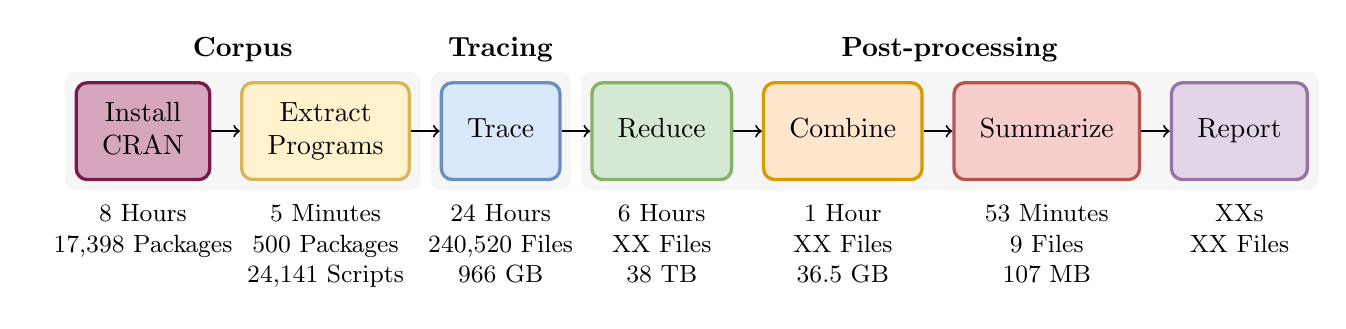
\begin{tikzpicture}
      \definecolor{maroon}{HTML}{D5A6BD}
      \definecolor{darkmaroon}{HTML}{741B47}
      \definecolor{yellow}{HTML}{FFF2CC}
      \definecolor{darkyellow}{HTML}{D6B656}
      \definecolor{blue}{HTML}{DAE8FC}
      \definecolor{darkblue}{HTML}{6C8EBF}
      \definecolor{green}{HTML}{D5E8D4}
      \definecolor{darkgreen}{HTML}{82B366}
      \definecolor{orange}{HTML}{FFE6CC}
      \definecolor{darkorange}{HTML}{D79B00}
      \definecolor{red}{HTML}{F8CECC}
      \definecolor{darkred}{HTML}{B85450}
      \definecolor{purple}{HTML}{E1D5E7}
      \definecolor{darkpurple}{HTML}{9673A6}
      \definecolor{gray}{HTML}{F5F5F5}

      \newcommand{\nodesep}[0]{0.030 \textwidth}
      \newcommand{\textsep}[0]{0.010 \textwidth}
      \newcommand{\backopacity}[0]{0.9}

      \newcommand{\nodename}[1]{\normalsize \begin{tabular}{c}#1\end{tabular}}
      \newcommand{\nodedesc}[1]{\small \begin{tabular}{c}#1\end{tabular}}

      \tikzstyle{block}     = [rectangle, rounded corners, minimum width=.08 \textwidth, minimum height=35pt]
      \tikzstyle{connector} = [line width=0.25mm, ->]

      \node [block, draw = darkmaroon, very thick, fill = maroon]                                (install)   {\nodename{Install\\CRAN}};
      \node [block, draw = darkyellow, very thick, fill = yellow, right = \nodesep of install  ] (extract)   {\nodename{Extract\\Programs}};
      \node [block, draw = darkblue,   very thick, fill = blue  , right = \nodesep of extract  ] (trace)     {\nodename{Trace}};
      \node [block, draw = darkgreen,  very thick, fill = green , right = \nodesep of trace    ] (reduce)    {\nodename{Reduce}};
      \node [block, draw = darkorange, very thick, fill = orange, right = \nodesep of reduce   ] (combine)   {\nodename{Combine}};
      \node [block, draw = darkred,    very thick, fill = red   , right = \nodesep of combine  ] (summarize) {\nodename{Summarize}};
      \node [block, draw = darkpurple, very thick, fill = purple, right = \nodesep of summarize] (report)    {\nodename{Report}};

      \draw [connector] (install)   edge (extract);
      \draw [connector] (extract)   edge (trace);
      \draw [connector] (trace)     edge (reduce);
      \draw [connector] (reduce)    edge (combine);
      \draw [connector] (combine)   edge (summarize);
      \draw [connector] (summarize) edge (report);

      \node [below = \textsep of install]   (installdesc)   {\nodedesc{8 Hours\\17,398 Packages}};
      \node [below = \textsep of extract]   (extractdesc)   {\nodedesc{5 Minutes\\500 Packages\\24,141 Scripts}};
      \node [below = \textsep of trace]     (tracedesc)     {\nodedesc{24 Hours\\240,520 Files\\966 GB}};
      \node [below = \textsep of reduce]    (reducedesc)    {\nodedesc{6 Hours\\XX Files\\38 TB}};
      \node [below = \textsep of combine]   (combinedesc)   {\nodedesc{1 Hour\\XX Files\\36.5 GB}};
      \node [below = \textsep of summarize] (summarizedesc) {\nodedesc{53 Minutes\\9 Files\\107 MB}};
      \node [below = \textsep of report]    (reportdesc)    {\nodedesc{XXs\\XX Files}};

      \begin{scope}[on background layer]
        \node[fit=(install) (extract), rectangle, rounded corners, fill=gray, fill opacity=\backopacity, label=above:\textbf{Corpus}]          (corpus) {};
        \node[fit=(trace),             rectangle, rounded corners, fill=gray, fill opacity=\backopacity, label=above:\textbf{Tracing}]         (exectrace) {};
        \node[fit=(reduce) (report),   rectangle, rounded corners, fill=gray, fill opacity=\backopacity, label=above:\textbf{Post-processing}] (postprocessing) {};
      \end{scope}
    \end{tikzpicture}
  }
  \caption{Analysis Pipeline}\label{ap}
\end{figure}

\subsection{Corpus}\label{sec:corpus}

A corpus of 500 packages with the most clients were selected from
CRAN~\cite{ligges2017} and Bioconductor~\cite{bioc} on the 26th of July 2021.
The packages have a total of 15,362 clients ranging from \c{ggplot2} with 2,669
clients all the way to \c{spatstat.linnet} with only 5. The packages have 2.2M
lines of R code and 2.7M lines of native code. Table~\ref{table:corpus}
summarizes the runnable code. Each test is run as a separate script. Examples
and vignettes are snippets of code embedded in the documentation. \lazr extracts
them into self-standing scripts. Typically, vignettes are longer examples with
input data, while examples are smaller code fragments.

\begin{wraptable}{r}{7cm}
  \vspace{-3mm}
  \small
  \centering
  \caption{Corpus}\label{table:corpus}
  \vspace{-3mm}
  \begin{tabular}{lrrr}
    \toprule
    &\bf Tests&\bf Examples&\bf Vignettes\\
    \midrule
    {Scripts}&5.8K&20.2K&631\\
    \midrule
    {LOC}&406.4K&207.0K&48.7K\\
    \bottomrule
  \end{tabular}
\end{wraptable}%%

There are 50,435 top-level functions, their distribution per packages is given
in Table~\ref{table:packsize}; 148 packages have 25 functions or less, and 12
packages with more than 500 functions. The largest package, \c{spatstat.geom},
has 886 functions. We observe 137.2M calls to these functions, their
distribution per function is in Fig.~\ref{fig:callDist}; 49\% of functions are
called more than ten times, while 16\% are called only once.

\begin{table}[!h]\small
  \caption{Package Size} \label{table:packsize}\centering
  \begin{tabular}{lr}\toprule
    \bf Functions&\bf Packages\\\midrule
    1--25&148\\
    26--50&98\\
    51--75&52\\
    76--100&33\\
    101--150&54\\
    151--200&34\\
    201--250&28\\\bottomrule
  \end{tabular}
  \quad\begin{tabular}{lr}\toprule
    \bf Functions&\bf Packages\\\midrule
    251--300&16\\
    301--400&14\\
    401--500&7\\
    501--600&5\\
    601--700&1\\
    701--800&4\\
    801--900&2\\\bottomrule
  \end{tabular}
\end{table}

The trace record 294M arguments, of those, close to 4M are missing, 19M are
$...$ and 271M are promises. These arguments correspond to 186K parameter
positions; 7\% of functions have no parameters, 19\% have 1, and 5\% have over
10, and 15 functions have over 50 parameters. Function
\c{rpart.plot::check.if.dot.arg.supported.by.rpart.rules} takes the cake with
122 parameters.

\begin{figure}[!h]  \centering
  % Created by tikzDevice version 0.12.3.1 on 2021-04-09 21:52:41
% !TEX encoding = UTF-8 Unicode
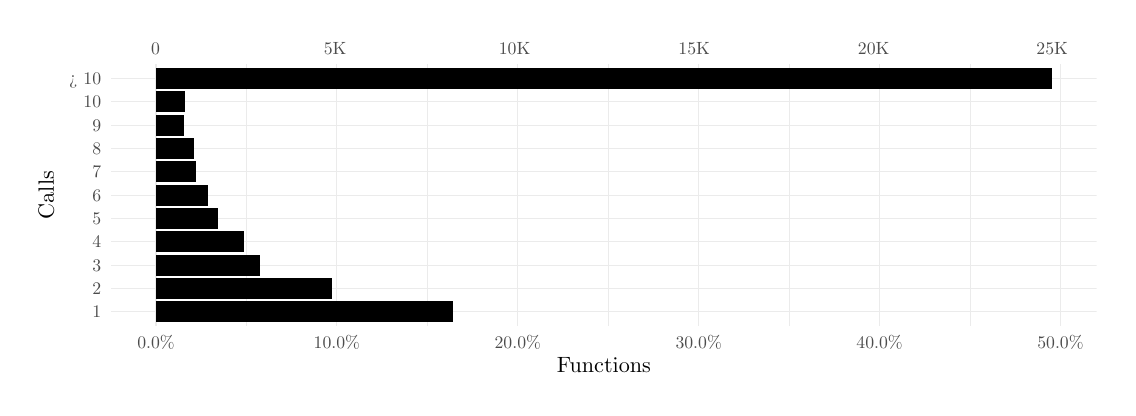
\begin{tikzpicture}[x=1pt,y=1pt]
\definecolor{fillColor}{RGB}{255,255,255}
\path[use as bounding box,fill=fillColor,fill opacity=0.00] (0,0) rectangle (390.26,130.09);
\begin{scope}
\path[clip] ( 30.17, 22.32) rectangle (386.26,116.83);
\definecolor{drawColor}{gray}{0.92}

\path[draw=drawColor,line width= 0.2pt,line join=round] ( 79.04, 22.32) --
	( 79.04,116.83);

\path[draw=drawColor,line width= 0.2pt,line join=round] (144.41, 22.32) --
	(144.41,116.83);

\path[draw=drawColor,line width= 0.2pt,line join=round] (209.77, 22.32) --
	(209.77,116.83);

\path[draw=drawColor,line width= 0.2pt,line join=round] (275.14, 22.32) --
	(275.14,116.83);

\path[draw=drawColor,line width= 0.2pt,line join=round] (340.51, 22.32) --
	(340.51,116.83);

\path[draw=drawColor,line width= 0.4pt,line join=round] ( 30.17, 27.38) --
	(386.26, 27.38);

\path[draw=drawColor,line width= 0.4pt,line join=round] ( 30.17, 35.82) --
	(386.26, 35.82);

\path[draw=drawColor,line width= 0.4pt,line join=round] ( 30.17, 44.26) --
	(386.26, 44.26);

\path[draw=drawColor,line width= 0.4pt,line join=round] ( 30.17, 52.70) --
	(386.26, 52.70);

\path[draw=drawColor,line width= 0.4pt,line join=round] ( 30.17, 61.14) --
	(386.26, 61.14);

\path[draw=drawColor,line width= 0.4pt,line join=round] ( 30.17, 69.58) --
	(386.26, 69.58);

\path[draw=drawColor,line width= 0.4pt,line join=round] ( 30.17, 78.01) --
	(386.26, 78.01);

\path[draw=drawColor,line width= 0.4pt,line join=round] ( 30.17, 86.45) --
	(386.26, 86.45);

\path[draw=drawColor,line width= 0.4pt,line join=round] ( 30.17, 94.89) --
	(386.26, 94.89);

\path[draw=drawColor,line width= 0.4pt,line join=round] ( 30.17,103.33) --
	(386.26,103.33);

\path[draw=drawColor,line width= 0.4pt,line join=round] ( 30.17,111.77) --
	(386.26,111.77);

\path[draw=drawColor,line width= 0.4pt,line join=round] ( 46.36, 22.32) --
	( 46.36,116.83);

\path[draw=drawColor,line width= 0.4pt,line join=round] (111.72, 22.32) --
	(111.72,116.83);

\path[draw=drawColor,line width= 0.4pt,line join=round] (177.09, 22.32) --
	(177.09,116.83);

\path[draw=drawColor,line width= 0.4pt,line join=round] (242.46, 22.32) --
	(242.46,116.83);

\path[draw=drawColor,line width= 0.4pt,line join=round] (307.82, 22.32) --
	(307.82,116.83);

\path[draw=drawColor,line width= 0.4pt,line join=round] (373.19, 22.32) --
	(373.19,116.83);
\definecolor{fillColor}{RGB}{0,0,0}

\path[fill=fillColor] ( 46.36,107.97) rectangle (370.07,115.57);

\path[fill=fillColor] ( 46.36, 23.58) rectangle (153.52, 31.18);

\path[fill=fillColor] ( 46.36, 99.53) rectangle ( 56.78,107.13);

\path[fill=fillColor] ( 46.36, 32.02) rectangle (109.88, 39.62);

\path[fill=fillColor] ( 46.36, 40.46) rectangle ( 83.98, 48.06);

\path[fill=fillColor] ( 46.36, 48.90) rectangle ( 78.12, 56.49);

\path[fill=fillColor] ( 46.36, 57.34) rectangle ( 68.81, 64.93);

\path[fill=fillColor] ( 46.36, 65.78) rectangle ( 65.03, 73.37);

\path[fill=fillColor] ( 46.36, 74.22) rectangle ( 60.74, 81.81);

\path[fill=fillColor] ( 46.36, 82.66) rectangle ( 60.20, 90.25);

\path[fill=fillColor] ( 46.36, 91.10) rectangle ( 56.47, 98.69);
\end{scope}
\begin{scope}
\path[clip] (  0.00,  0.00) rectangle (390.26,130.09);
\definecolor{drawColor}{gray}{0.30}

\node[text=drawColor,anchor=base,inner sep=0pt, outer sep=0pt, scale=  0.64] at ( 46.21,120.43) {0};

\node[text=drawColor,anchor=base,inner sep=0pt, outer sep=0pt, scale=  0.64] at (111.09,120.43) {5K};

\node[text=drawColor,anchor=base,inner sep=0pt, outer sep=0pt, scale=  0.64] at (175.96,120.43) {10K};

\node[text=drawColor,anchor=base,inner sep=0pt, outer sep=0pt, scale=  0.64] at (240.83,120.43) {15K};

\node[text=drawColor,anchor=base,inner sep=0pt, outer sep=0pt, scale=  0.64] at (305.70,120.43) {20K};

\node[text=drawColor,anchor=base,inner sep=0pt, outer sep=0pt, scale=  0.64] at (370.22,120.43) {25K};
\end{scope}
\begin{scope}
\path[clip] (  0.00,  0.00) rectangle (390.26,130.09);
\definecolor{drawColor}{gray}{0.30}

\node[text=drawColor,anchor=base east,inner sep=0pt, outer sep=0pt, scale=  0.64] at ( 26.57, 25.18) {1};

\node[text=drawColor,anchor=base east,inner sep=0pt, outer sep=0pt, scale=  0.64] at ( 26.57, 33.62) {2};

\node[text=drawColor,anchor=base east,inner sep=0pt, outer sep=0pt, scale=  0.64] at ( 26.57, 42.05) {3};

\node[text=drawColor,anchor=base east,inner sep=0pt, outer sep=0pt, scale=  0.64] at ( 26.57, 50.49) {4};

\node[text=drawColor,anchor=base east,inner sep=0pt, outer sep=0pt, scale=  0.64] at ( 26.57, 58.93) {5};

\node[text=drawColor,anchor=base east,inner sep=0pt, outer sep=0pt, scale=  0.64] at ( 26.57, 67.37) {6};

\node[text=drawColor,anchor=base east,inner sep=0pt, outer sep=0pt, scale=  0.64] at ( 26.57, 75.81) {7};

\node[text=drawColor,anchor=base east,inner sep=0pt, outer sep=0pt, scale=  0.64] at ( 26.57, 84.25) {8};

\node[text=drawColor,anchor=base east,inner sep=0pt, outer sep=0pt, scale=  0.64] at ( 26.57, 92.69) {9};

\node[text=drawColor,anchor=base east,inner sep=0pt, outer sep=0pt, scale=  0.64] at ( 26.57,101.13) {10};

\node[text=drawColor,anchor=base east,inner sep=0pt, outer sep=0pt, scale=  0.64] at ( 26.57,109.57) {> 10};
\end{scope}
\begin{scope}
\path[clip] (  0.00,  0.00) rectangle (390.26,130.09);
\definecolor{drawColor}{gray}{0.30}

\node[text=drawColor,anchor=base,inner sep=0pt, outer sep=0pt, scale=  0.64] at ( 46.36, 14.31) {0.0{\%}};

\node[text=drawColor,anchor=base,inner sep=0pt, outer sep=0pt, scale=  0.64] at (111.72, 14.31) {10.0{\%}};

\node[text=drawColor,anchor=base,inner sep=0pt, outer sep=0pt, scale=  0.64] at (177.09, 14.31) {20.0{\%}};

\node[text=drawColor,anchor=base,inner sep=0pt, outer sep=0pt, scale=  0.64] at (242.46, 14.31) {30.0{\%}};

\node[text=drawColor,anchor=base,inner sep=0pt, outer sep=0pt, scale=  0.64] at (307.82, 14.31) {40.0{\%}};

\node[text=drawColor,anchor=base,inner sep=0pt, outer sep=0pt, scale=  0.64] at (373.19, 14.31) {50.0{\%}};
\end{scope}
\begin{scope}
\path[clip] (  0.00,  0.00) rectangle (390.26,130.09);
\definecolor{drawColor}{RGB}{0,0,0}

\node[text=drawColor,anchor=base,inner sep=0pt, outer sep=0pt, scale=  0.80] at (208.22,  5.56) {Functions};
\end{scope}
\begin{scope}
\path[clip] (  0.00,  0.00) rectangle (390.26,130.09);
\definecolor{drawColor}{RGB}{0,0,0}

\node[text=drawColor,rotate= 90.00,anchor=base,inner sep=0pt, outer sep=0pt, scale=  0.80] at (  9.51, 69.58) {Calls};
\end{scope}
\end{tikzpicture}

  \caption{Call Distribution}\label{fig:callDist}
\end{figure}

\subsection{Inferred strictness signatures}\label{sec:results}

\lazr obtained data for 50,435 functions and 186K parameters. The results are
signals (M, U, S, R) for individual parameters. There were 9,100 parameters that
were marked M for meta-programmed. Table~\ref{table:strictdist} summarizes the
distribution of the combination of the other signals; note that functions and
packages can be counted in multiple rows as different parameters fall in
multiple categories. Rows can be interpreted as follows: the first row, for
instance, shows that 128K parameters coming from 44K functions and 489 packages
were not marked in any way. The second row shows that only 134 parameters
were marked R only for their use of reflective operations.

The data yields the following insights. First, the majority of parameters, 65\%,
are always evaluated, and the corresponding arguments do not perform
side-effects or reflective operations. They can become strict. Of the remaining,
there are 13\% of unevaluated parameters, the most significant potential source of
laziness. This is followed by 4\% of parameters whose arguments are marked S
only. The rest of the configurations are quite low. Another observation is that
rows marked R come from very few functions and packages.

\begin{table}
  \vspace{-3mm}
  \small
  \caption{Signature Summary} \label{table:strictdist}
  \centering
  \begin{tabular}{ccccccrrrrr}
    \toprule
    \bf ... & \bf M & \bf ? & \bf U & \bf S & \bf R & \multicolumn{2}{c}{\textbf{Parameters}} & \multicolumn{2}{c}{\textbf{Functions}}& \bf Packages\\
    \midrule
    \xmark{}&\xmark{}&\xmark{}&\xmark{}&\xmark{}&\xmark{}&148.4K&72.8\%&49.3K&93.4\%&489\\
    \xmark{}&\xmark{}&\xmark{}&\xmark{}&\xmark{}&\cmark{}&529&0.3\%&509&1\%&119\\
    \xmark{}&\xmark{}&\xmark{}&\xmark{}&\cmark{}&\xmark{}&1.3K&0.7\%&950&1.8\%&207\\
    \xmark{}&\xmark{}&\xmark{}&\xmark{}&\cmark{}&\cmark{}&76&0\%&74&0.1\%&22\\
    \xmark{}&\xmark{}&\xmark{}&\cmark{}&\xmark{}&\xmark{}&28.5K&14\%&12.4K&23.6\%&450\\
    \xmark{}&\xmark{}&\xmark{}&\cmark{}&\xmark{}&\cmark{}&33&0\%&32&0.1\%&24\\
    \xmark{}&\xmark{}&\xmark{}&\cmark{}&\cmark{}&\xmark{}&314&0.1\%&226&0.4\%&98\\
    \xmark{}&\xmark{}&\xmark{}&\cmark{}&\cmark{}&\cmark{}&9&0\%&9&0\%&5\\
    \rmark{}&\rmark{}&\cmark{}&\rmark{}&\rmark{}&\rmark{}&3.2K&1.6\%&1.7K&3.2\%&240\\
    \rmark{}&\cmark{}&\rmark{}&\rmark{}&\rmark{}&\rmark{}&1.3K&0.6\%&825&1.6\%&118\\
    \cmark{}&\rmark{}&\rmark{}&\rmark{}&\rmark{}&\rmark{}&20.0K&9.8\%&20.0K&37.9\%&430\\
    \bottomrule
  \end{tabular}
\end{table}


The inferred strictness signatures for library functions use these marks to
decide which arguments should be lazy and which should be strict. While any
parameter marked M \emph{must} be lazy, there is some freedom to decide for the
other combinations. Our evaluation will probe the different configurations and
show the error rates they may have.

\medskip

We now discuss the different sources of laziness in more detail.


\subsubsection{Metaprogramming}

\begin{wraptable}{r}{5.5cm}
  \small
  \centering
  \caption{Metaprogramming}\label{table:metaprogramming}
  \vspace{-3mm}
  \begin{tabular}{lrrr}
    \toprule
    &\bf R&\bf Native&\bf Total\\
    \midrule
    {Arguments}&\MetaCountArgumentsR&\MetaCountArgumentsNative&\MetaCountArgumentsTotal\\
    {Parameters}&\MetaCountParametersR&\MetaCountParametersNative&\MetaCountParametersTotal\\
    {Functions}&\MetaCountFunctionsR&\MetaCountFunctionsNative&\MetaCountFunctionsTotal\\
    {Packages}&\MetaCountPackagesR&\MetaCountPackagesNative&\MetaCountPackagesTotal\\
    \bottomrule
  \end{tabular}
\end{wraptable}


Meta-programming tracks calls to \code{substitute} (from R) and \code{PREXPR}
(from native code). Table~\ref{table:metaprogramming} shows the number of
arguments, parameters, functions, and packages using metaprogramming. Out of
\AG{total number of arguments} model arguments, \MetaCountArgumentsTotal were
meta-programmed. This results in \MetaCountParametersTotal lazy parameters from
\MetaCountFunctionsTotal functions of \MetaCountPackagesTotal packages. While
more arguments are metaprogrammed using \code{substitute} than \code{PREXPR},
they correspond to fewer parameters.

For a discussion of the use of \code{substitute} we refer the reader to
\citet{oopsla19b}. We elaborate on \code{PREXPR} since it was not addressed
there. This macro is used by many packages to extract a promise's expression for
ad-hoc evaluation strategies. We found its uses in packages like \code{lazyeval}
and \code{rlang}. The \code{rlang} package particularly stands out because it
provides its own API for meta-programming. The \code{PREXPR} macro is also used
by the builtin functions of the GNU R interpreter, a canonical example is the
\code{missing} function to check if an argument was provided. Unlike user
packages, these uses of \code{PREXPR} don't require the corresponding arguments
to be lazily evaluated. Hence, parameters metaprogrammed using \code{PREXPR}
from GNU R interpreter are not made lazy. They are also not included in
Table~\ref{table:metaprogramming}.


\subsubsection{Missing Arguments}

\begin{wraptable}{r}{6cm}
  \small
  \centering
  \caption{Missing}\label{table:missing}
  \vspace{-3mm}
  \begin{tabular}{lrrr}
    \toprule
    &\bf Sometimes&\bf Always&\bf Total\\
    \midrule
    {Argments}&\MissingSometimesCountArguments&\MissingAlwaysCountArguments&\MissingTotalCountArguments\\
    {Parameters}&\MissingSometimesCountParameters&\MissingAlwaysCountParameters&\MissingTotalCountParameters\\
    {Functions}&\MissingSometimesCountFunctions&\MissingAlwaysCountFunctions&\MissingTotalCountFunctions\\
    {Packages}&\MissingSometimesCountPackages&\MissingAlwaysCountPackages&\MissingTotalCountPackages\\
    \bottomrule
  \end{tabular}
\end{wraptable}

Of the 294M total arguments in our corpus, \MissingTotalCountArguments arguments
were missing. This excludes the \c{...} and metaprogrammed parameters which
could also be missing, but are separately discussed above. These
\MissingTotalCountArguments arguments correspond to \MissingTotalCountParameters
parameters. Arguments to \MissingAlwaysCountParameters of these parameters are
always missing. These parameters are classified as \always, in contrast to the
\MissingSometimesCountParameters \sometimes parameters which are sometimes
passed an argument. The distribution of these two categories is presented in
Table~\ref{table:missing}. The \always parameters are treated as lazy, whereas
the \sometimes parameters are treated as lazy if they don't evaluate the
arguments passed to them at least once. These parameters are dealt like other
parameters in Section~\ref{subsubsection:unevaluted_arguments} discussed below.

The example below shows an example of \always missing parameter. The \c{names}
argument was missing in all the calls to this function defined in the \c{rlang}
package. Since the function does not use this argument, it is present presumably
for future evolution or backwards compatibility.

\begin{lstlisting}
new_environments <- function(envs, names) {
  stopifnot(is_list(envs))
  structure(envs,
            names = map_chr(unname(envs), env_name),
            class = "rlang_envs")
}
\end{lstlisting}

The example below shows an example of \sometimes missing parameter. The
\c{linewidth} argument was missing in some calls to this function defined in the
\c{base64enc} package. The function assigns a default value of \c{0L} to
\c{linewidth} if it is missing.

\begin{lstlisting}
base64encode <- function(what, linewidth, newline) {
  linewidth <- if (missing(linewidth) || !is.numeric(linewidth) ||
                  length(linewidth) < 1L) 0L
               else as.integer(linewidth[1L])
    ...
}

\end{lstlisting}


\subsubsection{Unevaluated Arguments} \label{subsubsection:unevaluted_arguments}

\begin{wraptable}{r}{6cm}
  \small
  \centering
  \caption{Unevaluated}\label{table:unevaluated}
  \vspace{-3mm}
  \begin{tabular}{lrrr}
    \toprule
    &\bf Sometimes&\bf Never&\bf Total\\
    \midrule
    {Parameters}&\UnevaluatedSometimesCountParameters&\UnevaluatedNeverCountParameters&\UnevaluatedTotalCountParameters\\
    {Functions}&\UnevaluatedSometimesCountFunctions&\UnevaluatedNeverCountFunctions&\UnevaluatedTotalCountFunctions\\
    {Packages}&\UnevaluatedSometimesCountPackages&\UnevaluatedNeverCountPackages&\UnevaluatedTotalCountPackages\\
    \bottomrule
  \end{tabular}
\end{wraptable}

Of the 294M total arguments in our corpus, \UnevaluatedTotalCountArguments of
promises were not evaluated. They correspond to \UnevaluatedTotalCountParameters
parameters from \UnevaluatedTotalCountFunctions functions of
\UnevaluatedTotalCountPackages packages. We can classify these parameters into
two categories: parameters that are \sometimes evaluated and parameters that are
\never evaluated. Table~\ref{table:unevaluated} presents the number of
parameters, functions, and packages in these two categories. There are
\UnevaluatedSometimesCountParameters \sometimes parameters and
\UnevaluatedNeverCountParameters \never parameters. These may correspond to code
paths not exercised or to dummy parameters.
%
A common pattern is the following:
%
\begin{lstlisting}
 lazyeval::%||% <- function(x, y) if(is.null(x)) y else x
\end{lstlisting}
%
This function evaluates \code{y} only if \code{x} is \code{NULL}, making
\code{y} a \sometimes parameter.
\noindent
Another pattern is to delay the evaluation of a parameter.

\begin{lstlisting}
 glue::on_package_load <- function(pkg, expr) {
   if (isNamespaceLoaded(pkg)) { expr }
   else {
     thunk <- function(...) expr
     setHook(packageEvent(pkg, "onLoad"), thunk)
   }
 }
\end{lstlisting}
%
Here, \code{expr} may be delayed until \code{pkg} is loaded. Thus, \code{expr}
should not be evaluated strictly.
%
S3 generics result in many \sometimes and \never parameters. These functions
dynamically dispatch to a specific implementation based on the argument's class.
In the following example, the first argument is always evaluated, but \code{n}
and \code{m} are only evaluated sometimes and \code{r} never.
%
\begin{lstlisting}
 abind::acorn <- function(x, n=6, m=5, r=1, ...) UseMethod('acorn')
\end{lstlisting}
\noindent
One source of \never parameters is when a set of functions implements a common
interface, but not all functions need all parameters. The \code{proxy} package
defines over a dozen methods with the interface \code{function(a,b,c,d,n)} that
compute different proximity metrics using a subset of the arguments.

Arguments can be \never by design; \code{tail} is not defined for
\code{tbl_lazy} objects and throws an error when called.
\begin{lstlisting}
 dbplyr::tail.tbl_lazy <- function(x, n = 6L, ...)
   stop("tail() is not supported by sql sources", call.=FALSE)
\end{lstlisting}
%
\never parameters can also represent an erroneous condition that would not
happen in a correct program. The following function fails if its argument does
not have the correct type. In all observed calls, \code{signal}
went  unused because \code{e} had the right type.
\begin{lstlisting}
 codetools::checkSymOrString <- function(e, signal = stop) {
   type <- typeof(e)
   if (type == "symbol" || type == "character") e
   else signal("not a symbol or string")
 }
\end{lstlisting}

\subsubsection{Side-Effects}

Of all the promises observed by \lazr, only 0.5\% perform side-effects. Many
side-effects are benign for our purposes because they happen in environments
that are scoped by the evaluation of the promise, and the side-effects are ignored.

\begin{table}[!h]  \vspace{-3mm}  \small
  \caption{Effects} \label{table:effects} \centering
  \begin{tabular}{llllll}    \toprule
    \textbf{Effect}&\textbf{Count}&\textbf{Arguments}&\textbf{Parameters}&\textbf{Functions}&\textbf{Packages}\\    \midrule
    L&3.7M&1.2M&5.6K&3.7K&359\\
    D&1.1M&159.0K&3.0K&2.6K&319\\
    A&235.8K&122.7K&511.0&487.0&109\\
    R&2.8K&718.0&27.0&24.0&10\\    \bottomrule
  \end{tabular}
\end{table}

\noindent
Table~\ref{table:effects} counts lookups (L), definitions (D), assignments (A),
and removals (R), and the arguments, parameters, functions, and packages directly
responsible for those effects. Lookups are the most common cause for making
arguments lazy. This is followed by definitions and assignments. Removing
bindings from environments is not a common operation.
%
Comparing the number of events in this table against the total number of events,
we narrow 89B variable lookups down to 3.7M, 20B definitions to 1.1M, and 7B
assignments to 235K.

\begin{wraptable}{r}{5cm}
  \vspace{-3mm}
  \small
  \caption{Effect Sequence} \label{table:effectseq}
  \centering
  \begin{tabular}{lll}
    \toprule
    \textbf{Sequence}&\textbf{Arguments}\\
    \midrule
    -&99.5\%\\
    L+&0.41\%\\
    D+&0.04\%\\
    A+&0.03\%\\
    (L+D+)+&0.01\%\\
    \bottomrule
  \end{tabular}
\end{wraptable}

An argument can perform a combination of effects during evaluation.
Table~\ref{table:effectseq} shows the sequence of operations performed by the
arguments in our corpus. The majority of arguments, 99.5\% to be precise, do not
perform any relevant effect. 0.41\% only perform a sequence of lookups, 0.04\%
perform a sequence of definitions, 0.03\% perform assignments, and 0.01\%
perform a sequence of lookups and definitions. From this, we conclude that
the majority of arguments have a simple pattern of events.

A common source of non-local writes is the \c{shiny} package used for building
interactive web applications. Consider the call to \code{bindEvent} which
attaches an observer expression to an event. The observer performs a non-local
side-effect using \code{<<-}, this is a common way to update the global state.
%
\begin{lstlisting}
 bindEvent(trigger(), x=observe({vals <<- c(vals, val())}))
\end{lstlisting}
%
\noindent
Another source of non-local writes occurs in the \code{withr} package. It
provides functions to evaluate code in a temporarily modified global state. These
code blocks assign their result in the current scope. In the following example, a
side-effecting expression is passed to \code{with\_seed} which changes the
random number generation seed.
%
\begin{lstlisting}
 with_seed(seed <- sample.int(.Machine$integer.max, 1), runif(5))
\end{lstlisting}
%
\noindent
Many side-effects occur in test cases written with the \code{testthat} library.
The global state is modified temporarily to test its effect on the function
under consideration.
%
Another common pattern is when the result of an intermediate computation is
assigned to a variable for subsequent use. In the call below, the intermediate
result is assigned to \code{x} before being passed on to the
\code{as.data.table} function.
%
\begin{lstlisting}
 as.data.table(x <- as.character(sample(letters, 5)))
\end{lstlisting}
%
\noindent
Deleting a variable from an environment is done with the \code{rm} function.
The following function computes the number of rows of a data frame and assigns
it to a variable \code{.N} in the caller's environment. Eventually, it removes the
variable.
%
\begin{lstlisting}
 [.data.table <- function (x, i, j, ...) {
   assign(".N", nrow(x), envir=parent.frame(), inherits=FALSE)
   if (remove.N) rm(list=".N", envir=parent.frame())
   ...
\end{lstlisting}
\noindent
Lastly, \code{rlang} defines a function \code{env_bind} which can be used to
create and remove bindings from an environment. When passed with the value
\code{zap()}, it removes the corresponding symbol from the environment. It uses
the C function \code{R_removeVarFromFrame}.

\subsubsection{Reflection}
Reflective code is brittle. The following example shows that code that looks up
its call stack is sensitive to small implementation changes, such as the
addition of a call to an identity function. The evaluation of \c x and \c y will
yield different results as the latter is executing within the \c{id} function.
%
\begin{lstlisting}
 id <- function(a) a
 f <- function(x, y) { x; id(y); }
 f(as.environment(-1), as.environment(-1))
\end{lstlisting}
%
\noindent
This can transitively affect the strictness of other parameters. If \code{f} is
called from \code{g} as shown below, we will have to make \code{g} non-strict in
\code{u} and \code{v}. Their results depend upon how they are evaluated inside
\code{f}.

\begin{lstlisting}
 g <- function(u, v) { f(u, v) }
 g(as.environment(-1), as.environment(-1))
\end{lstlisting}
%
\noindent
R provides other functions for reflective stack access, \code{parent.frame} and
\code{sys.frame}; these are less brittle as they access frames relative to the
promise's creation environment.

\begin{wraptable}{r}{5.5cm}
  \small
  \centering
  \caption{Reflection}\label{table:reflection}
  \vspace{-3mm}
  \begin{tabular}{lrrr}
    \toprule
    &\bf Direct&\bf Transitive&\bf Total\\
    \midrule
    {Arguments}&\RefCountArgumentsDirect&\RefCountArgumentsTransitive&\RefCountArgumentsTotal\\
    {Parameters}&\RefCountParametersDirect&\RefCountParametersTransitive&\RefCountParametersTotal\\
    {Functions}&\RefCountFunctionsDirect&\RefCountFunctionsTransitive&\RefCountFunctionsTotal\\
    {Packages}&\RefCountPackagesDirect&\RefCountPackagesTransitive&\RefCountPackagesTotal\\
    \bottomrule
  \end{tabular}
\end{wraptable}

Table~\ref{table:reflection} presents the number of arguments that call
\code{as.environment(-1)} and \code{pos.to.env(-1)} directly or transitively.
This excludes the cases where the argument is also metaprogrammed. Two
parameters from two functions, \code{R.oo::.getFunctionByName}, and
\code{backports:::get0} call these functions directly.
%
The first searches for a function by name in different scopes. Its argument has
a default value of \code{as.environment(-1)}.
%
\begin{lstlisting}
 R.oo:::.getFunctionByName <- function(..., callEnvir = as.environment(-1L), ...) {
   envirT <- callEnvir
   ...
\end{lstlisting}
%

\subsection{Robustness of inferred signatures} \label{Evaluation:Robustness}

\begin{figure}[th!]
  \centering
  \scalebox{0.85}{
    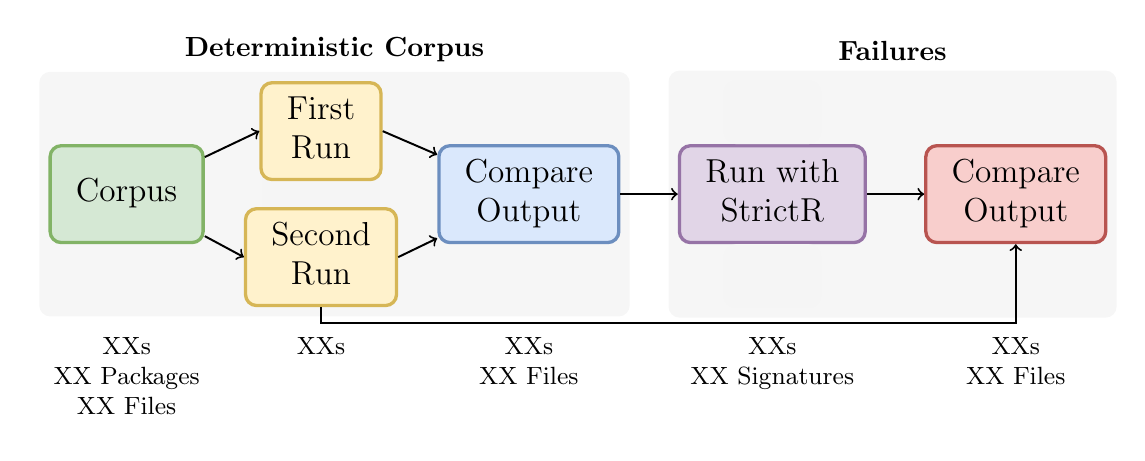
\begin{tikzpicture}

      \definecolor{gray}{HTML}{F5F5F5}
      \definecolor{green}{HTML}{D5E8D4}
      \definecolor{darkgreen}{HTML}{82B366}
      \definecolor{yellow}{HTML}{FFF2CC}
      \definecolor{darkyellow}{HTML}{D6B656}
      \definecolor{blue}{HTML}{DAE8FC}
      \definecolor{darkblue}{HTML}{6C8EBF}
      \definecolor{purple}{HTML}{E1D5E7}
      \definecolor{darkpurple}{HTML}{9673A6}
      \definecolor{red}{HTML}{F8CECC}
      \definecolor{darkred}{HTML}{B85450}

      \tikzstyle{block}      = [rectangle, rounded corners, minimum width=.12 \textwidth, minimum height=35pt]
      \tikzstyle{dummyblock} = [rectangle, rounded corners, minimum width=.10 \textwidth, minimum height=22pt]

      \tikzstyle{connector} = [line width=0.25mm, ->]

      \newcommand{\nodesep}[0]{0.060 \textwidth}
      \newcommand{\dummynodesep}[0]{8mm}
      \newcommand{\textsep}[0]{10mm}
      \newcommand{\backopacity}[0]{0.9}

      \newcommand{\nodename}[1]{\large \begin{tabular}{c}#1\end{tabular}}
      \newcommand{\nodedesc}[1]{\small \begin{tabular}{c}#1\end{tabular}}

      \node [block,      draw = darkgreen,  very thick, fill = green]                                                           (corpus)            {\nodename{Corpus}};
      \node [block,      draw = gray,       very thick, fill = gray,   right = \nodesep of corpus]                              (dummyrun)          {};
      \node [block,      draw = darkyellow, very thick, fill = yellow, above = \dummynodesep of dummyrun.north, anchor = north] (runone)            {\nodename{First\\Run}};
      \node [block,      draw = darkyellow, very thick, fill = yellow, below = \dummynodesep of dummyrun.south, anchor = south] (runtwo)            {\nodename{Second\\Run}};
      \node [block,      draw = darkblue,   very thick, fill = blue,   right = \nodesep of dummyrun]                            (outone)            {\nodename{Compare\\Output}};
      \node [block,      draw = darkpurple, very thick, fill = purple, right = \nodesep of outone]                              (strictrun)         {\nodename{Run with\\StrictR}};
      \node [dummyblock, draw = gray,       very thick, fill = gray,   above = 0mm of strictrun.north]                          (dummystrictrun)    {};
      \node [dummyblock, draw = gray,       very thick, fill = gray,   below = 0mm of strictrun.south]                          (dummystrictruntwo) {};
      \node [block,      draw = darkred,    very thick, fill = red,    right = \nodesep of strictrun]                           (outtwo)            {\nodename{Compare\\Output}};

      \draw [connector] (corpus)       -- (runone.west);
      \draw [connector] (corpus)       -- (runtwo.west);
      \draw [connector] (runone.east)  -- (outone);
      \draw [connector] (runtwo.east)  -- (outone);
      \draw [connector] (outone)       -- (strictrun);
      \draw [connector] (strictrun)    -- (outtwo);
      \draw [connector] (runtwo.south) -- ++(0, -0.2) -| ($(runtwo) !1.0! (outtwo.south)$);

      \node [below = \textsep of corpus]    (corpusdesc)     {\nodedesc{XXs\\XX Packages\\XX Files}};
      \node [below = \textsep of dummyrun]  (rundesc)        {\nodedesc{XXs}};
      \node [below = \textsep of outone]    (outonedesc)     {\nodedesc{XXs\\XX Files}};
      \node [below = \textsep of strictrun] (strictrundesc)  {\nodedesc{XXs\\XX Signatures}};
      \node [below = \textsep of outtwo]    (outtwodesc)     {\nodedesc{XXs\\XX Files}};

      \begin{scope}[on background layer]
        \node[fit=(corpus) (runone) (runtwo) (outone),                       rectangle, rounded corners, fill=gray, fill opacity=\backopacity, label=above:\textbf{Deterministic Corpus}] (detcorpus) {};
        \node[fit=(strictrun) (dummystrictrun) (dummystrictruntwo) (outtwo), rectangle, rounded corners, fill=gray, fill opacity=\backopacity, label=above:\textbf{Failures}] (failures) {};
      \end{scope}

    \end{tikzpicture}
  }
  \caption{Validation Pipeline}\label{fig:validationPipeline}
\end{figure}

In this section, we evaluate the robustness of strictness signatures generated
by \lazr. This is done by running scripts extracted from 2,000 client packages of
our corpus. These packages have 4.5M lines of R code and 4.7M lines of native
code. Table ~\ref{table:clientcorpus} gives the number of scripts and lines of code
exercised.

\begin{wraptable}{r}{6cm}  \vspace{-3mm}  \small  \centering
  \caption{Client Corpus}\label{table:clientcorpus}  \vspace{-3mm}
  \begin{tabular}{lrrr}    \toprule
    &\bf Tests&\bf Examples&\bf Vignettes\\
    \midrule
    {Scripts} &9.8K&41.1K&1.7K\\
    \midrule
    {LOC} &751.2K&348.8K&112.3K\\    \bottomrule
  \end{tabular}
\end{wraptable}%%

Using \lazr, we extracted 52K scripts from the clients. From these, we filtered
scripts whose output was non-deterministic, leaving us with 42K scripts. The
goal of the next step is to validate if, after applying strictness signatures,
they produce identical outputs.

Comparing the output of scripts is standard practice in the R community for
detecting regressions. There may be a difference in execution that does not
manifest in the output; this may hide some errors, so the results reported here
should be considered a lower bound.

\begin{wraptable}{r}{5cm}
  \small
  \caption{Strictness Failure} \label{table:strictfail}
  \centering
  \begin{tabular}{lc|ll}
    \toprule
    \#&\textbf{Configuration}&\multicolumn{2}{c}{\textbf{Failures}}\\
    \midrule
    0&$+U+S+R$&239&0.56\%\\
    1&$+U+S-R$&234&0.55\%\\
    2&$+U-S+R$&1922&4.51\%\\
    3&$+U-S-R$&6625&15.54\%\\
    4&$-U+S+R$&610&1.43\%\\
    5&$-U+S-R$&616&1.44\%\\
    6&$-U-S+R$&2319&5.44\%\\
    7&$-U-S-R$&7158&16.79\%\\
    \bottomrule
  \end{tabular}
\end{wraptable}

Table~\ref{table:strictfail} reports on the eight configurations we evaluated.
For each row in the table, we ran all 42K scripts and counted the number of
differences from expected outputs. Each row corresponds to a different set of
strictness signatures for the corpus. The 9K parameters that were inferred to be
meta-programmed (M) are always lazy. The 128K parameters that were not marked
were always strict. For the 36K remaining parameters (those with a combination
of U, S, R), each row represents a different strictness setting.

For each configuration, we report the number and percentage of failing programs.
The \emph{+} sign indicates the corresponding parameter is lazy and \emph{-}
means strict. For example, in the $+U+S+R$ configuration, any parameter marked
as either U, S or R, is lazy, whereas the configuration $+U+S-R$ means that any
parameter marked U or S must be lazy, and the configuration $-U+S+R$ means that
parameters marked S and R must be lazy.

\cconfig 0 is the laziest of the configurations; only 239 scripts out of 42K
have erroneous outputs. These errors come from some of the
unmarked parameters. Consider, for instance, a library function \c f that was
always called without side-effects during inference and for which there is a
side-effecting client. \lazr would mark that function as strict, but the client
may be able to observe the semantic difference. Luckily, this is quite rare.

All other configurations are strictly stricter, and thus are likely to experience
more errors. The case of \config 1 is surprising, as making arguments reflective
hides 5 errors. This is an outlier that should be elided.

In the extreme, \config 7 makes all parameters marked either U, S, or R strict.
This leads to 16\% of failures which is rather high. This suggests a substantial
amount of accidental laziness which can be observed.

One takeaway from this evaluation is that unevaluated parameters (U) have only a
small impact on correctness, while S and R are the sources of most errors.

From the results, we conclude that using \config 0 as the starting point for
migration is the safest. The first attempt at removing laziness at scale can rely on
this signature configuration. Next, reflective and unevaluated arguments can be
made strict without a significant increase in failure rate. Side-effecting
arguments result in many failures.


\section{Performance Experiment}\label{sec:rsh}

Our hypothesis is that eager semantics lead to faster programs. This might
surprise readers who expect that call-by-need i can avoid unnecessary
computation. Delaying computations is complex and hinders performance in two
ways. First, it leads to more allocations of promises. Second, it obstructs
compiler analyses and optimizations. We expect the hypothesis to hold for a
just-in-time compiler that uses advanced optimizations like \Rsh. In particular,
we expect: (1) eager semantics to improve performance of most benchmarks, for
both tiers of \Rsh; (2) a portion of the speedup to come from reduced garbage
collection; (3) and an additional speedup due to improved compiler
optimizations. We present our evidence in support of (1) and (3), and partial
evidence for (2).

\paragraph{Methodology}
We conducted limit-study experiment to assess the highest achievable performance
by removing maximum possible promises, we do this on small benchmarks that we
manually annotated. We picked a subset of the \Rsh benchmark suite which
includes one variant of each benchmark. Only a handful of functions, such as
\lstinline{tryCatch}, had to be kept lazy. Experiments are run on a dedicated
benchmarking machine, with all background tasks disabled. The system features an
Intel i7-6700K CPU, stepping 3, microcode 0xe2 with 4 cores and 8 threads. The
system has 32 GB of RAM and is running Ubuntu 18.04 on a 4.15.0-136 Linux
kernel. For ease of use, experiments are built as containers, based on Ubuntu
20.04, and executed on the Docker runtime 20.10.5, build 55c4c88. We verified
the overhead introduced by the containerization to be uniform. All measurements
are recorded repeatedly and we keep a historical record to spot unstable
behavior. This led us to exclude the \lstinline{convolution} benchmark as it
appears to have a bi-modal performance profile, likely caused by the LLVM
backend.
Performance measurements are gathered by running $t_e$ invocations of \Rsh on
each benchmark. Within each invocation we measure the execution time of $t_i$
in-process invocations. For each invocation, the first 5 in-process iterations
are discarded to exclude warmup behavior. Aggregate numbers are reported as the
speedup over the arithmetic mean of the execution times. Multiple speedup
numbers are averaged using a geometric mean. To establish a baseline we measured
the speedup of \Rsh over GNU R, on our subsetted benchmark suite with parameters
$t_e = 1, t_i = 15$. We found a mean speedup of \speedupRsh, ranging between
\speedupRshMin and \speedupRshMax.

\paragraph{Speedup}

\begin{figure}[h]
  \centering % Created by tikzDevice version 0.12.3.1 on 2021-04-16 11:39:57
% !TEX encoding = UTF-8 Unicode
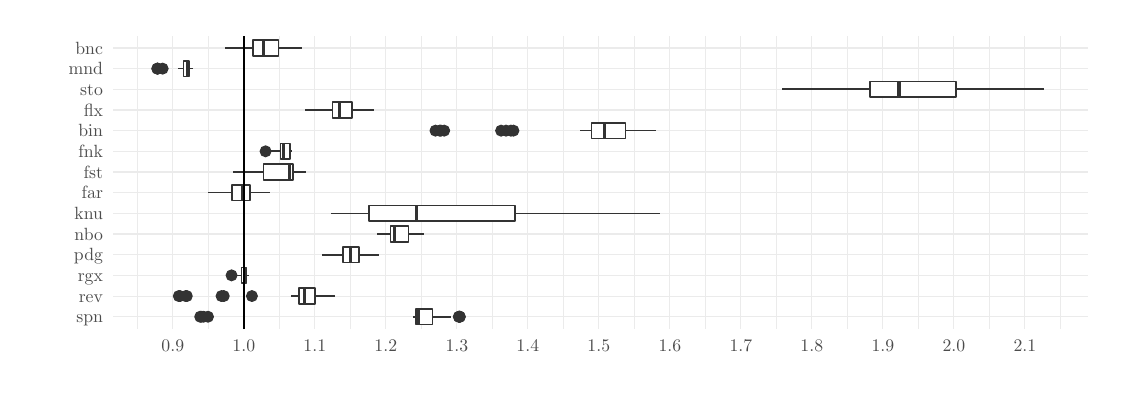
\begin{tikzpicture}[x=1pt,y=1pt]
\definecolor{fillColor}{RGB}{255,255,255}
\path[use as bounding box,fill=fillColor,fill opacity=0.00] (0,0) rectangle (390.26,130.09);
\begin{scope}
\path[clip] ( 30.80, 21.16) rectangle (383.14,127.24);
\definecolor{drawColor}{gray}{0.92}

\path[draw=drawColor,line width= 0.2pt,line join=round] ( 39.61, 21.16) --
	( 39.61,127.24);

\path[draw=drawColor,line width= 0.2pt,line join=round] ( 65.27, 21.16) --
	( 65.27,127.24);

\path[draw=drawColor,line width= 0.2pt,line join=round] ( 90.93, 21.16) --
	( 90.93,127.24);

\path[draw=drawColor,line width= 0.2pt,line join=round] (116.58, 21.16) --
	(116.58,127.24);

\path[draw=drawColor,line width= 0.2pt,line join=round] (142.24, 21.16) --
	(142.24,127.24);

\path[draw=drawColor,line width= 0.2pt,line join=round] (167.90, 21.16) --
	(167.90,127.24);

\path[draw=drawColor,line width= 0.2pt,line join=round] (193.55, 21.16) --
	(193.55,127.24);

\path[draw=drawColor,line width= 0.2pt,line join=round] (219.21, 21.16) --
	(219.21,127.24);

\path[draw=drawColor,line width= 0.2pt,line join=round] (244.87, 21.16) --
	(244.87,127.24);

\path[draw=drawColor,line width= 0.2pt,line join=round] (270.52, 21.16) --
	(270.52,127.24);

\path[draw=drawColor,line width= 0.2pt,line join=round] (296.18, 21.16) --
	(296.18,127.24);

\path[draw=drawColor,line width= 0.2pt,line join=round] (321.84, 21.16) --
	(321.84,127.24);

\path[draw=drawColor,line width= 0.2pt,line join=round] (347.50, 21.16) --
	(347.50,127.24);

\path[draw=drawColor,line width= 0.2pt,line join=round] (373.15, 21.16) --
	(373.15,127.24);

\path[draw=drawColor,line width= 0.4pt,line join=round] ( 30.80, 25.64) --
	(383.14, 25.64);

\path[draw=drawColor,line width= 0.4pt,line join=round] ( 30.80, 33.11) --
	(383.14, 33.11);

\path[draw=drawColor,line width= 0.4pt,line join=round] ( 30.80, 40.59) --
	(383.14, 40.59);

\path[draw=drawColor,line width= 0.4pt,line join=round] ( 30.80, 48.06) --
	(383.14, 48.06);

\path[draw=drawColor,line width= 0.4pt,line join=round] ( 30.80, 55.53) --
	(383.14, 55.53);

\path[draw=drawColor,line width= 0.4pt,line join=round] ( 30.80, 63.00) --
	(383.14, 63.00);

\path[draw=drawColor,line width= 0.4pt,line join=round] ( 30.80, 70.47) --
	(383.14, 70.47);

\path[draw=drawColor,line width= 0.4pt,line join=round] ( 30.80, 77.94) --
	(383.14, 77.94);

\path[draw=drawColor,line width= 0.4pt,line join=round] ( 30.80, 85.41) --
	(383.14, 85.41);

\path[draw=drawColor,line width= 0.4pt,line join=round] ( 30.80, 92.88) --
	(383.14, 92.88);

\path[draw=drawColor,line width= 0.4pt,line join=round] ( 30.80,100.35) --
	(383.14,100.35);

\path[draw=drawColor,line width= 0.4pt,line join=round] ( 30.80,107.82) --
	(383.14,107.82);

\path[draw=drawColor,line width= 0.4pt,line join=round] ( 30.80,115.29) --
	(383.14,115.29);

\path[draw=drawColor,line width= 0.4pt,line join=round] ( 30.80,122.76) --
	(383.14,122.76);

\path[draw=drawColor,line width= 0.4pt,line join=round] ( 52.44, 21.16) --
	( 52.44,127.24);

\path[draw=drawColor,line width= 0.4pt,line join=round] ( 78.10, 21.16) --
	( 78.10,127.24);

\path[draw=drawColor,line width= 0.4pt,line join=round] (103.75, 21.16) --
	(103.75,127.24);

\path[draw=drawColor,line width= 0.4pt,line join=round] (129.41, 21.16) --
	(129.41,127.24);

\path[draw=drawColor,line width= 0.4pt,line join=round] (155.07, 21.16) --
	(155.07,127.24);

\path[draw=drawColor,line width= 0.4pt,line join=round] (180.72, 21.16) --
	(180.72,127.24);

\path[draw=drawColor,line width= 0.4pt,line join=round] (206.38, 21.16) --
	(206.38,127.24);

\path[draw=drawColor,line width= 0.4pt,line join=round] (232.04, 21.16) --
	(232.04,127.24);

\path[draw=drawColor,line width= 0.4pt,line join=round] (257.70, 21.16) --
	(257.70,127.24);

\path[draw=drawColor,line width= 0.4pt,line join=round] (283.35, 21.16) --
	(283.35,127.24);

\path[draw=drawColor,line width= 0.4pt,line join=round] (309.01, 21.16) --
	(309.01,127.24);

\path[draw=drawColor,line width= 0.4pt,line join=round] (334.67, 21.16) --
	(334.67,127.24);

\path[draw=drawColor,line width= 0.4pt,line join=round] (360.32, 21.16) --
	(360.32,127.24);
\definecolor{drawColor}{gray}{0.20}
\definecolor{fillColor}{gray}{0.20}

\path[draw=drawColor,line width= 0.4pt,line join=round,line cap=round,fill=fillColor] (156.15, 25.64) circle (  1.96);

\path[draw=drawColor,line width= 0.4pt,line join=round,line cap=round,fill=fillColor] (156.12, 25.64) circle (  1.96);

\path[draw=drawColor,line width= 0.4pt,line join=round,line cap=round,fill=fillColor] (155.99, 25.64) circle (  1.96);

\path[draw=drawColor,line width= 0.4pt,line join=round,line cap=round,fill=fillColor] (155.93, 25.64) circle (  1.96);

\path[draw=drawColor,line width= 0.4pt,line join=round,line cap=round,fill=fillColor] (155.78, 25.64) circle (  1.96);

\path[draw=drawColor,line width= 0.4pt,line join=round,line cap=round,fill=fillColor] ( 65.16, 25.64) circle (  1.96);

\path[draw=drawColor,line width= 0.4pt,line join=round,line cap=round,fill=fillColor] ( 63.52, 25.64) circle (  1.96);

\path[draw=drawColor,line width= 0.4pt,line join=round,line cap=round,fill=fillColor] ( 62.73, 25.64) circle (  1.96);

\path[draw=drawColor,line width= 0.4pt,line join=round,line cap=round,fill=fillColor] ( 62.34, 25.64) circle (  1.96);

\path[draw=drawColor,line width= 0.6pt,line join=round] (146.25, 25.64) -- (152.79, 25.64);

\path[draw=drawColor,line width= 0.6pt,line join=round] (140.37, 25.64) -- (139.26, 25.64);
\definecolor{fillColor}{RGB}{255,255,255}

\path[draw=drawColor,line width= 0.6pt,line join=round,line cap=round,fill=fillColor] (146.25, 22.84) --
	(140.37, 22.84) --
	(140.37, 28.45) --
	(146.25, 28.45) --
	(146.25, 22.84) --
	cycle;

\path[draw=drawColor,line width= 1.1pt,line join=round] (141.25, 22.84) -- (141.25, 28.45);
\definecolor{fillColor}{gray}{0.20}

\path[draw=drawColor,line width= 0.4pt,line join=round,line cap=round,fill=fillColor] ( 81.03, 33.11) circle (  1.96);

\path[draw=drawColor,line width= 0.4pt,line join=round,line cap=round,fill=fillColor] ( 70.85, 33.11) circle (  1.96);

\path[draw=drawColor,line width= 0.4pt,line join=round,line cap=round,fill=fillColor] ( 70.05, 33.11) circle (  1.96);

\path[draw=drawColor,line width= 0.4pt,line join=round,line cap=round,fill=fillColor] ( 57.50, 33.11) circle (  1.96);

\path[draw=drawColor,line width= 0.4pt,line join=round,line cap=round,fill=fillColor] ( 57.11, 33.11) circle (  1.96);

\path[draw=drawColor,line width= 0.4pt,line join=round,line cap=round,fill=fillColor] ( 55.03, 33.11) circle (  1.96);

\path[draw=drawColor,line width= 0.4pt,line join=round,line cap=round,fill=fillColor] ( 54.61, 33.11) circle (  1.96);

\path[draw=drawColor,line width= 0.6pt,line join=round] (103.83, 33.11) -- (110.91, 33.11);

\path[draw=drawColor,line width= 0.6pt,line join=round] ( 98.16, 33.11) -- ( 95.23, 33.11);
\definecolor{fillColor}{RGB}{255,255,255}

\path[draw=drawColor,line width= 0.6pt,line join=round,line cap=round,fill=fillColor] (103.83, 30.31) --
	( 98.16, 30.31) --
	( 98.16, 35.92) --
	(103.83, 35.92) --
	(103.83, 30.31) --
	cycle;

\path[draw=drawColor,line width= 1.1pt,line join=round] (100.11, 30.31) -- (100.11, 35.92);
\definecolor{fillColor}{gray}{0.20}

\path[draw=drawColor,line width= 0.4pt,line join=round,line cap=round,fill=fillColor] ( 73.67, 40.59) circle (  1.96);

\path[draw=drawColor,line width= 0.6pt,line join=round] ( 79.10, 40.59) -- ( 79.80, 40.59);

\path[draw=drawColor,line width= 0.6pt,line join=round] ( 77.25, 40.59) -- ( 74.95, 40.59);
\definecolor{fillColor}{RGB}{255,255,255}

\path[draw=drawColor,line width= 0.6pt,line join=round,line cap=round,fill=fillColor] ( 79.10, 37.78) --
	( 77.25, 37.78) --
	( 77.25, 43.39) --
	( 79.10, 43.39) --
	( 79.10, 37.78) --
	cycle;

\path[draw=drawColor,line width= 1.1pt,line join=round] ( 78.68, 37.78) -- ( 78.68, 43.39);

\path[draw=drawColor,line width= 0.6pt,line join=round] (119.62, 48.06) -- (126.98, 48.06);

\path[draw=drawColor,line width= 0.6pt,line join=round] (113.92, 48.06) -- (106.44, 48.06);

\path[draw=drawColor,line width= 0.6pt,line join=round,line cap=round,fill=fillColor] (119.62, 45.25) --
	(113.92, 45.25) --
	(113.92, 50.86) --
	(119.62, 50.86) --
	(119.62, 45.25) --
	cycle;

\path[draw=drawColor,line width= 1.1pt,line join=round] (116.71, 45.25) -- (116.71, 50.86);

\path[draw=drawColor,line width= 0.6pt,line join=round] (137.64, 55.53) -- (143.32, 55.53);

\path[draw=drawColor,line width= 0.6pt,line join=round] (131.11, 55.53) -- (126.10, 55.53);

\path[draw=drawColor,line width= 0.6pt,line join=round,line cap=round,fill=fillColor] (137.64, 52.72) --
	(131.11, 52.72) --
	(131.11, 58.33) --
	(137.64, 58.33) --
	(137.64, 52.72) --
	cycle;

\path[draw=drawColor,line width= 1.1pt,line join=round] (132.52, 52.72) -- (132.52, 58.33);

\path[draw=drawColor,line width= 0.6pt,line join=round] (176.13, 63.00) -- (228.50, 63.00);

\path[draw=drawColor,line width= 0.6pt,line join=round] (123.24, 63.00) -- (109.43, 63.00);

\path[draw=drawColor,line width= 0.6pt,line join=round,line cap=round,fill=fillColor] (176.13, 60.19) --
	(123.24, 60.19) --
	(123.24, 65.80) --
	(176.13, 65.80) --
	(176.13, 60.19) --
	cycle;

\path[draw=drawColor,line width= 1.1pt,line join=round] (140.40, 60.19) -- (140.40, 65.80);

\path[draw=drawColor,line width= 0.6pt,line join=round] ( 80.43, 70.47) -- ( 87.42, 70.47);

\path[draw=drawColor,line width= 0.6pt,line join=round] ( 73.78, 70.47) -- ( 65.12, 70.47);

\path[draw=drawColor,line width= 0.6pt,line join=round,line cap=round,fill=fillColor] ( 80.43, 67.66) --
	( 73.78, 67.66) --
	( 73.78, 73.27) --
	( 80.43, 73.27) --
	( 80.43, 67.66) --
	cycle;

\path[draw=drawColor,line width= 1.1pt,line join=round] ( 77.51, 67.66) -- ( 77.51, 73.27);

\path[draw=drawColor,line width= 0.6pt,line join=round] ( 95.85, 77.94) -- (100.61, 77.94);

\path[draw=drawColor,line width= 0.6pt,line join=round] ( 85.22, 77.94) -- ( 74.17, 77.94);

\path[draw=drawColor,line width= 0.6pt,line join=round,line cap=round,fill=fillColor] ( 95.85, 75.14) --
	( 85.22, 75.14) --
	( 85.22, 80.74) --
	( 95.85, 80.74) --
	( 95.85, 75.14) --
	cycle;

\path[draw=drawColor,line width= 1.1pt,line join=round] ( 94.47, 75.14) -- ( 94.47, 80.74);
\definecolor{fillColor}{gray}{0.20}

\path[draw=drawColor,line width= 0.4pt,line join=round,line cap=round,fill=fillColor] ( 85.96, 85.41) circle (  1.96);

\path[draw=drawColor,line width= 0.6pt,line join=round] ( 94.71, 85.41) -- ( 95.48, 85.41);

\path[draw=drawColor,line width= 0.6pt,line join=round] ( 91.33, 85.41) -- ( 87.02, 85.41);
\definecolor{fillColor}{RGB}{255,255,255}

\path[draw=drawColor,line width= 0.6pt,line join=round,line cap=round,fill=fillColor] ( 94.71, 82.61) --
	( 91.33, 82.61) --
	( 91.33, 88.21) --
	( 94.71, 88.21) --
	( 94.71, 82.61) --
	cycle;

\path[draw=drawColor,line width= 1.1pt,line join=round] ( 92.53, 82.61) -- ( 92.53, 88.21);
\definecolor{fillColor}{gray}{0.20}

\path[draw=drawColor,line width= 0.4pt,line join=round,line cap=round,fill=fillColor] (175.53, 92.88) circle (  1.96);

\path[draw=drawColor,line width= 0.4pt,line join=round,line cap=round,fill=fillColor] (174.60, 92.88) circle (  1.96);

\path[draw=drawColor,line width= 0.4pt,line join=round,line cap=round,fill=fillColor] (172.86, 92.88) circle (  1.96);

\path[draw=drawColor,line width= 0.4pt,line join=round,line cap=round,fill=fillColor] (171.07, 92.88) circle (  1.96);

\path[draw=drawColor,line width= 0.4pt,line join=round,line cap=round,fill=fillColor] (150.51, 92.88) circle (  1.96);

\path[draw=drawColor,line width= 0.4pt,line join=round,line cap=round,fill=fillColor] (149.30, 92.88) circle (  1.96);

\path[draw=drawColor,line width= 0.4pt,line join=round,line cap=round,fill=fillColor] (148.89, 92.88) circle (  1.96);

\path[draw=drawColor,line width= 0.4pt,line join=round,line cap=round,fill=fillColor] (147.36, 92.88) circle (  1.96);

\path[draw=drawColor,line width= 0.6pt,line join=round] (215.97, 92.88) -- (227.06, 92.88);

\path[draw=drawColor,line width= 0.6pt,line join=round] (203.77, 92.88) -- (199.42, 92.88);
\definecolor{fillColor}{RGB}{255,255,255}

\path[draw=drawColor,line width= 0.6pt,line join=round,line cap=round,fill=fillColor] (215.97, 90.08) --
	(203.77, 90.08) --
	(203.77, 95.68) --
	(215.97, 95.68) --
	(215.97, 90.08) --
	cycle;

\path[draw=drawColor,line width= 1.1pt,line join=round] (208.57, 90.08) -- (208.57, 95.68);

\path[draw=drawColor,line width= 0.6pt,line join=round] (117.23,100.35) -- (125.27,100.35);

\path[draw=drawColor,line width= 0.6pt,line join=round] (110.12,100.35) -- (100.09,100.35);

\path[draw=drawColor,line width= 0.6pt,line join=round,line cap=round,fill=fillColor] (117.23, 97.55) --
	(110.12, 97.55) --
	(110.12,103.15) --
	(117.23,103.15) --
	(117.23, 97.55) --
	cycle;

\path[draw=drawColor,line width= 1.1pt,line join=round] (112.68, 97.55) -- (112.68,103.15);

\path[draw=drawColor,line width= 0.6pt,line join=round] (335.48,107.82) -- (367.13,107.82);

\path[draw=drawColor,line width= 0.6pt,line join=round] (304.34,107.82) -- (272.46,107.82);

\path[draw=drawColor,line width= 0.6pt,line join=round,line cap=round,fill=fillColor] (335.48,105.02) --
	(304.34,105.02) --
	(304.34,110.62) --
	(335.48,110.62) --
	(335.48,105.02) --
	cycle;

\path[draw=drawColor,line width= 1.1pt,line join=round] (314.85,105.02) -- (314.85,110.62);
\definecolor{fillColor}{gray}{0.20}

\path[draw=drawColor,line width= 0.4pt,line join=round,line cap=round,fill=fillColor] ( 48.77,115.29) circle (  1.96);

\path[draw=drawColor,line width= 0.4pt,line join=round,line cap=round,fill=fillColor] ( 47.00,115.29) circle (  1.96);

\path[draw=drawColor,line width= 0.4pt,line join=round,line cap=round,fill=fillColor] ( 46.92,115.29) circle (  1.96);

\path[draw=drawColor,line width= 0.4pt,line join=round,line cap=round,fill=fillColor] ( 46.81,115.29) circle (  1.96);

\path[draw=drawColor,line width= 0.6pt,line join=round] ( 58.27,115.29) -- ( 59.68,115.29);

\path[draw=drawColor,line width= 0.6pt,line join=round] ( 56.36,115.29) -- ( 54.49,115.29);
\definecolor{fillColor}{RGB}{255,255,255}

\path[draw=drawColor,line width= 0.6pt,line join=round,line cap=round,fill=fillColor] ( 58.27,112.49) --
	( 56.36,112.49) --
	( 56.36,118.09) --
	( 58.27,118.09) --
	( 58.27,112.49) --
	cycle;

\path[draw=drawColor,line width= 1.1pt,line join=round] ( 57.71,112.49) -- ( 57.71,118.09);

\path[draw=drawColor,line width= 0.6pt,line join=round] ( 90.59,122.76) -- ( 99.03,122.76);

\path[draw=drawColor,line width= 0.6pt,line join=round] ( 81.46,122.76) -- ( 71.38,122.76);

\path[draw=drawColor,line width= 0.6pt,line join=round,line cap=round,fill=fillColor] ( 90.59,119.96) --
	( 81.46,119.96) --
	( 81.46,125.56) --
	( 90.59,125.56) --
	( 90.59,119.96) --
	cycle;

\path[draw=drawColor,line width= 1.1pt,line join=round] ( 85.21,119.96) -- ( 85.21,125.56);
\definecolor{drawColor}{RGB}{0,0,0}

\path[draw=drawColor,line width= 0.6pt,line join=round] ( 78.10, 21.16) -- ( 78.10,127.24);
\end{scope}
\begin{scope}
\path[clip] (  0.00,  0.00) rectangle (390.26,130.09);
\definecolor{drawColor}{gray}{0.30}

\node[text=drawColor,anchor=base east,inner sep=0pt, outer sep=0pt, scale=  0.64] at ( 27.20, 23.44) {spn};

\node[text=drawColor,anchor=base east,inner sep=0pt, outer sep=0pt, scale=  0.64] at ( 27.20, 30.91) {rev};

\node[text=drawColor,anchor=base east,inner sep=0pt, outer sep=0pt, scale=  0.64] at ( 27.20, 38.38) {rgx};

\node[text=drawColor,anchor=base east,inner sep=0pt, outer sep=0pt, scale=  0.64] at ( 27.20, 45.85) {pdg};

\node[text=drawColor,anchor=base east,inner sep=0pt, outer sep=0pt, scale=  0.64] at ( 27.20, 53.32) {nbo};

\node[text=drawColor,anchor=base east,inner sep=0pt, outer sep=0pt, scale=  0.64] at ( 27.20, 60.79) {knu};

\node[text=drawColor,anchor=base east,inner sep=0pt, outer sep=0pt, scale=  0.64] at ( 27.20, 68.26) {far};

\node[text=drawColor,anchor=base east,inner sep=0pt, outer sep=0pt, scale=  0.64] at ( 27.20, 75.73) {fst};

\node[text=drawColor,anchor=base east,inner sep=0pt, outer sep=0pt, scale=  0.64] at ( 27.20, 83.20) {fnk};

\node[text=drawColor,anchor=base east,inner sep=0pt, outer sep=0pt, scale=  0.64] at ( 27.20, 90.67) {bin};

\node[text=drawColor,anchor=base east,inner sep=0pt, outer sep=0pt, scale=  0.64] at ( 27.20, 98.14) {flx};

\node[text=drawColor,anchor=base east,inner sep=0pt, outer sep=0pt, scale=  0.64] at ( 27.20,105.61) {sto};

\node[text=drawColor,anchor=base east,inner sep=0pt, outer sep=0pt, scale=  0.64] at ( 27.20,113.08) {mnd};

\node[text=drawColor,anchor=base east,inner sep=0pt, outer sep=0pt, scale=  0.64] at ( 27.20,120.55) {bnc};
\end{scope}
\begin{scope}
\path[clip] (  0.00,  0.00) rectangle (390.26,130.09);
\definecolor{drawColor}{gray}{0.30}

\node[text=drawColor,anchor=base,inner sep=0pt, outer sep=0pt, scale=  0.64] at ( 52.44, 13.15) {0.9};

\node[text=drawColor,anchor=base,inner sep=0pt, outer sep=0pt, scale=  0.64] at ( 78.10, 13.15) {1.0};

\node[text=drawColor,anchor=base,inner sep=0pt, outer sep=0pt, scale=  0.64] at (103.75, 13.15) {1.1};

\node[text=drawColor,anchor=base,inner sep=0pt, outer sep=0pt, scale=  0.64] at (129.41, 13.15) {1.2};

\node[text=drawColor,anchor=base,inner sep=0pt, outer sep=0pt, scale=  0.64] at (155.07, 13.15) {1.3};

\node[text=drawColor,anchor=base,inner sep=0pt, outer sep=0pt, scale=  0.64] at (180.72, 13.15) {1.4};

\node[text=drawColor,anchor=base,inner sep=0pt, outer sep=0pt, scale=  0.64] at (206.38, 13.15) {1.5};

\node[text=drawColor,anchor=base,inner sep=0pt, outer sep=0pt, scale=  0.64] at (232.04, 13.15) {1.6};

\node[text=drawColor,anchor=base,inner sep=0pt, outer sep=0pt, scale=  0.64] at (257.70, 13.15) {1.7};

\node[text=drawColor,anchor=base,inner sep=0pt, outer sep=0pt, scale=  0.64] at (283.35, 13.15) {1.8};

\node[text=drawColor,anchor=base,inner sep=0pt, outer sep=0pt, scale=  0.64] at (309.01, 13.15) {1.9};

\node[text=drawColor,anchor=base,inner sep=0pt, outer sep=0pt, scale=  0.64] at (334.67, 13.15) {2.0};

\node[text=drawColor,anchor=base,inner sep=0pt, outer sep=0pt, scale=  0.64] at (360.32, 13.15) {2.1};
\end{scope}
\end{tikzpicture}

  \caption{Speedup} \label{fig:speedup}
\end{figure}

First, we compare \Rsh against \rshstrict. This experiment estimates the
end-to-end improvement on performance that a change to eager semantics in the R
language would have on \Rsh. The execution times were measured with $t_e = 4,
t_i = 25$. \autoref{fig:speedup} shows a boxplot for the speedups of \rshstrict
along the X-axis, normalized with respect to \Rsh (lazy). Outliers are
represented by black dots. Overall, we observe a mean speedup of
\speedupRshStrict, ranging from \speedupRshStrictMin to \speedupRshStrictMax.
For \speedupRshStrictSignificant out of \benchmarkSuiteSize benchmarks we
measure a significant increase in performance.
%
\begin{figure}[h]
  \centering
  % Created by tikzDevice version 0.12.3.1 on 2021-04-14 13:17:10
% !TEX encoding = UTF-8 Unicode
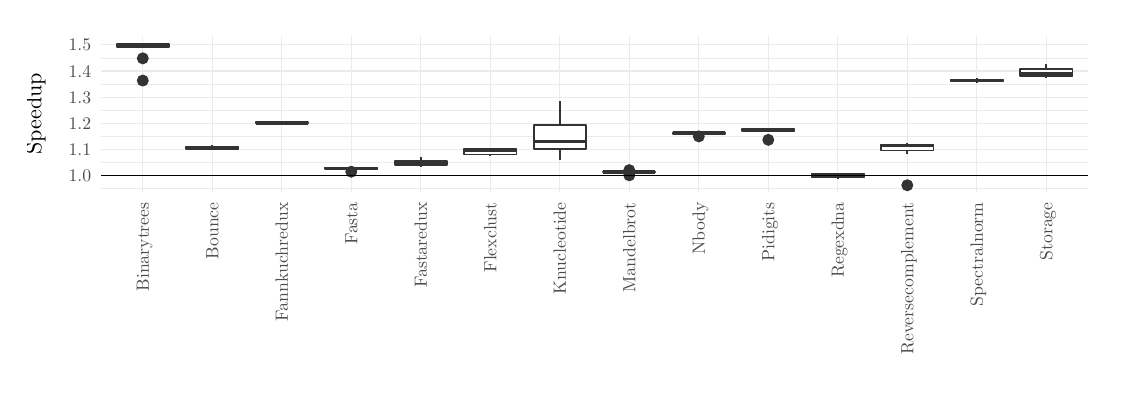
\begin{tikzpicture}[x=1pt,y=1pt]
\definecolor{fillColor}{RGB}{255,255,255}
\path[use as bounding box,fill=fillColor,fill opacity=0.00] (0,0) rectangle (390.26,130.09);
\begin{scope}
\path[clip] ( 26.53, 70.57) rectangle (383.14,127.24);
\definecolor{drawColor}{gray}{0.92}

\path[draw=drawColor,line width= 0.2pt,line join=round] ( 26.53, 71.98) --
	(383.14, 71.98);

\path[draw=drawColor,line width= 0.2pt,line join=round] ( 26.53, 81.42) --
	(383.14, 81.42);

\path[draw=drawColor,line width= 0.2pt,line join=round] ( 26.53, 90.85) --
	(383.14, 90.85);

\path[draw=drawColor,line width= 0.2pt,line join=round] ( 26.53,100.29) --
	(383.14,100.29);

\path[draw=drawColor,line width= 0.2pt,line join=round] ( 26.53,109.72) --
	(383.14,109.72);

\path[draw=drawColor,line width= 0.2pt,line join=round] ( 26.53,119.16) --
	(383.14,119.16);

\path[draw=drawColor,line width= 0.4pt,line join=round] ( 26.53, 76.70) --
	(383.14, 76.70);

\path[draw=drawColor,line width= 0.4pt,line join=round] ( 26.53, 86.14) --
	(383.14, 86.14);

\path[draw=drawColor,line width= 0.4pt,line join=round] ( 26.53, 95.57) --
	(383.14, 95.57);

\path[draw=drawColor,line width= 0.4pt,line join=round] ( 26.53,105.00) --
	(383.14,105.00);

\path[draw=drawColor,line width= 0.4pt,line join=round] ( 26.53,114.44) --
	(383.14,114.44);

\path[draw=drawColor,line width= 0.4pt,line join=round] ( 26.53,123.87) --
	(383.14,123.87);

\path[draw=drawColor,line width= 0.4pt,line join=round] ( 41.60, 70.57) --
	( 41.60,127.24);

\path[draw=drawColor,line width= 0.4pt,line join=round] ( 66.71, 70.57) --
	( 66.71,127.24);

\path[draw=drawColor,line width= 0.4pt,line join=round] ( 91.83, 70.57) --
	( 91.83,127.24);

\path[draw=drawColor,line width= 0.4pt,line join=round] (116.94, 70.57) --
	(116.94,127.24);

\path[draw=drawColor,line width= 0.4pt,line join=round] (142.05, 70.57) --
	(142.05,127.24);

\path[draw=drawColor,line width= 0.4pt,line join=round] (167.17, 70.57) --
	(167.17,127.24);

\path[draw=drawColor,line width= 0.4pt,line join=round] (192.28, 70.57) --
	(192.28,127.24);

\path[draw=drawColor,line width= 0.4pt,line join=round] (217.39, 70.57) --
	(217.39,127.24);

\path[draw=drawColor,line width= 0.4pt,line join=round] (242.51, 70.57) --
	(242.51,127.24);

\path[draw=drawColor,line width= 0.4pt,line join=round] (267.62, 70.57) --
	(267.62,127.24);

\path[draw=drawColor,line width= 0.4pt,line join=round] (292.74, 70.57) --
	(292.74,127.24);

\path[draw=drawColor,line width= 0.4pt,line join=round] (317.85, 70.57) --
	(317.85,127.24);

\path[draw=drawColor,line width= 0.4pt,line join=round] (342.96, 70.57) --
	(342.96,127.24);

\path[draw=drawColor,line width= 0.4pt,line join=round] (368.08, 70.57) --
	(368.08,127.24);
\definecolor{drawColor}{gray}{0.20}
\definecolor{fillColor}{gray}{0.20}

\path[draw=drawColor,line width= 0.4pt,line join=round,line cap=round,fill=fillColor] ( 41.60,119.00) circle (  1.96);

\path[draw=drawColor,line width= 0.4pt,line join=round,line cap=round,fill=fillColor] ( 41.60,110.98) circle (  1.96);

\path[draw=drawColor,line width= 0.6pt,line join=round] ( 41.60,124.07) -- ( 41.60,124.66);

\path[draw=drawColor,line width= 0.6pt,line join=round] ( 41.60,123.05) -- ( 41.60,123.02);
\definecolor{fillColor}{RGB}{255,255,255}

\path[draw=drawColor,line width= 0.6pt,line join=round,line cap=round,fill=fillColor] ( 32.18,124.07) --
	( 32.18,123.05) --
	( 51.02,123.05) --
	( 51.02,124.07) --
	( 32.18,124.07) --
	cycle;

\path[draw=drawColor,line width= 1.1pt,line join=round] ( 32.18,123.28) -- ( 51.02,123.28);

\path[draw=drawColor,line width= 0.6pt,line join=round] ( 66.71, 87.10) -- ( 66.71, 87.62);

\path[draw=drawColor,line width= 0.6pt,line join=round] ( 66.71, 86.23) -- ( 66.71, 85.92);

\path[draw=drawColor,line width= 0.6pt,line join=round,line cap=round,fill=fillColor] ( 57.30, 87.10) --
	( 57.30, 86.23) --
	( 76.13, 86.23) --
	( 76.13, 87.10) --
	( 57.30, 87.10) --
	cycle;

\path[draw=drawColor,line width= 1.1pt,line join=round] ( 57.30, 86.67) -- ( 76.13, 86.67);

\path[draw=drawColor,line width= 0.6pt,line join=round] ( 91.83, 96.08) -- ( 91.83, 96.51);

\path[draw=drawColor,line width= 0.6pt,line join=round] ( 91.83, 95.52) -- ( 91.83, 95.13);

\path[draw=drawColor,line width= 0.6pt,line join=round,line cap=round,fill=fillColor] ( 82.41, 96.08) --
	( 82.41, 95.52) --
	(101.24, 95.52) --
	(101.24, 96.08) --
	( 82.41, 96.08) --
	cycle;

\path[draw=drawColor,line width= 1.1pt,line join=round] ( 82.41, 95.65) -- (101.24, 95.65);
\definecolor{fillColor}{gray}{0.20}

\path[draw=drawColor,line width= 0.4pt,line join=round,line cap=round,fill=fillColor] (116.94, 78.04) circle (  1.96);

\path[draw=drawColor,line width= 0.6pt,line join=round] (116.94, 79.62) -- (116.94, 80.13);

\path[draw=drawColor,line width= 0.6pt,line join=round] (116.94, 79.07) -- (116.94, 78.60);
\definecolor{fillColor}{RGB}{255,255,255}

\path[draw=drawColor,line width= 0.6pt,line join=round,line cap=round,fill=fillColor] (107.52, 79.62) --
	(107.52, 79.07) --
	(126.36, 79.07) --
	(126.36, 79.62) --
	(107.52, 79.62) --
	cycle;

\path[draw=drawColor,line width= 1.1pt,line join=round] (107.52, 79.28) -- (126.36, 79.28);

\path[draw=drawColor,line width= 0.6pt,line join=round] (142.05, 81.94) -- (142.05, 83.46);

\path[draw=drawColor,line width= 0.6pt,line join=round] (142.05, 80.49) -- (142.05, 79.85);

\path[draw=drawColor,line width= 0.6pt,line join=round,line cap=round,fill=fillColor] (132.64, 81.94) --
	(132.64, 80.49) --
	(151.47, 80.49) --
	(151.47, 81.94) --
	(132.64, 81.94) --
	cycle;

\path[draw=drawColor,line width= 1.1pt,line join=round] (132.64, 81.42) -- (151.47, 81.42);

\path[draw=drawColor,line width= 0.6pt,line join=round] (167.17, 86.16) -- (167.17, 86.56);

\path[draw=drawColor,line width= 0.6pt,line join=round] (167.17, 84.31) -- (167.17, 83.69);

\path[draw=drawColor,line width= 0.6pt,line join=round,line cap=round,fill=fillColor] (157.75, 86.16) --
	(157.75, 84.31) --
	(176.59, 84.31) --
	(176.59, 86.16) --
	(157.75, 86.16) --
	cycle;

\path[draw=drawColor,line width= 1.1pt,line join=round] (157.75, 85.66) -- (176.59, 85.66);

\path[draw=drawColor,line width= 0.6pt,line join=round] (192.28, 94.98) -- (192.28,103.56);

\path[draw=drawColor,line width= 0.6pt,line join=round] (192.28, 86.21) -- (192.28, 82.24);

\path[draw=drawColor,line width= 0.6pt,line join=round,line cap=round,fill=fillColor] (182.86, 94.98) --
	(182.86, 86.21) --
	(201.70, 86.21) --
	(201.70, 94.98) --
	(182.86, 94.98) --
	cycle;

\path[draw=drawColor,line width= 1.1pt,line join=round] (182.86, 89.08) -- (201.70, 89.08);
\definecolor{fillColor}{gray}{0.20}

\path[draw=drawColor,line width= 0.4pt,line join=round,line cap=round,fill=fillColor] (217.39, 78.61) circle (  1.96);

\path[draw=drawColor,line width= 0.4pt,line join=round,line cap=round,fill=fillColor] (217.39, 76.74) circle (  1.96);

\path[draw=drawColor,line width= 0.6pt,line join=round] (217.39, 78.09) -- (217.39, 78.13);

\path[draw=drawColor,line width= 0.6pt,line join=round] (217.39, 77.86) -- (217.39, 77.59);
\definecolor{fillColor}{RGB}{255,255,255}

\path[draw=drawColor,line width= 0.6pt,line join=round,line cap=round,fill=fillColor] (207.98, 78.09) --
	(207.98, 77.86) --
	(226.81, 77.86) --
	(226.81, 78.09) --
	(207.98, 78.09) --
	cycle;

\path[draw=drawColor,line width= 1.1pt,line join=round] (207.98, 77.94) -- (226.81, 77.94);
\definecolor{fillColor}{gray}{0.20}

\path[draw=drawColor,line width= 0.4pt,line join=round,line cap=round,fill=fillColor] (242.51, 90.80) circle (  1.96);

\path[draw=drawColor,line width= 0.6pt,line join=round] (242.51, 92.21) -- (242.51, 92.32);

\path[draw=drawColor,line width= 0.6pt,line join=round] (242.51, 91.78) -- (242.51, 91.16);
\definecolor{fillColor}{RGB}{255,255,255}

\path[draw=drawColor,line width= 0.6pt,line join=round,line cap=round,fill=fillColor] (233.09, 92.21) --
	(233.09, 91.78) --
	(251.93, 91.78) --
	(251.93, 92.21) --
	(233.09, 92.21) --
	cycle;

\path[draw=drawColor,line width= 1.1pt,line join=round] (233.09, 92.07) -- (251.93, 92.07);
\definecolor{fillColor}{gray}{0.20}

\path[draw=drawColor,line width= 0.4pt,line join=round,line cap=round,fill=fillColor] (267.62, 89.56) circle (  1.96);

\path[draw=drawColor,line width= 0.6pt,line join=round] (267.62, 93.46) -- (267.62, 93.69);

\path[draw=drawColor,line width= 0.6pt,line join=round] (267.62, 92.73) -- (267.62, 92.57);
\definecolor{fillColor}{RGB}{255,255,255}

\path[draw=drawColor,line width= 0.6pt,line join=round,line cap=round,fill=fillColor] (258.20, 93.46) --
	(258.20, 92.73) --
	(277.04, 92.73) --
	(277.04, 93.46) --
	(258.20, 93.46) --
	cycle;

\path[draw=drawColor,line width= 1.1pt,line join=round] (258.20, 93.29) -- (277.04, 93.29);

\path[draw=drawColor,line width= 0.6pt,line join=round] (292.74, 77.36) -- (292.74, 77.50);

\path[draw=drawColor,line width= 0.6pt,line join=round] (292.74, 75.93) -- (292.74, 75.31);

\path[draw=drawColor,line width= 0.6pt,line join=round,line cap=round,fill=fillColor] (283.32, 77.36) --
	(283.32, 75.93) --
	(302.15, 75.93) --
	(302.15, 77.36) --
	(283.32, 77.36) --
	cycle;

\path[draw=drawColor,line width= 1.1pt,line join=round] (283.32, 76.68) -- (302.15, 76.68);
\definecolor{fillColor}{gray}{0.20}

\path[draw=drawColor,line width= 0.4pt,line join=round,line cap=round,fill=fillColor] (317.85, 73.15) circle (  1.96);

\path[draw=drawColor,line width= 0.6pt,line join=round] (317.85, 87.82) -- (317.85, 88.27);

\path[draw=drawColor,line width= 0.6pt,line join=round] (317.85, 85.75) -- (317.85, 84.30);
\definecolor{fillColor}{RGB}{255,255,255}

\path[draw=drawColor,line width= 0.6pt,line join=round,line cap=round,fill=fillColor] (308.43, 87.82) --
	(308.43, 85.75) --
	(327.27, 85.75) --
	(327.27, 87.82) --
	(308.43, 87.82) --
	cycle;

\path[draw=drawColor,line width= 1.1pt,line join=round] (308.43, 87.41) -- (327.27, 87.41);

\path[draw=drawColor,line width= 0.6pt,line join=round] (342.96,111.40) -- (342.96,111.74);

\path[draw=drawColor,line width= 0.6pt,line join=round] (342.96,110.58) -- (342.96,109.92);

\path[draw=drawColor,line width= 0.6pt,line join=round,line cap=round,fill=fillColor] (333.55,111.40) --
	(333.55,110.58) --
	(352.38,110.58) --
	(352.38,111.40) --
	(333.55,111.40) --
	cycle;

\path[draw=drawColor,line width= 1.1pt,line join=round] (333.55,111.17) -- (352.38,111.17);

\path[draw=drawColor,line width= 0.6pt,line join=round] (368.08,115.10) -- (368.08,116.89);

\path[draw=drawColor,line width= 0.6pt,line join=round] (368.08,112.52) -- (368.08,111.75);

\path[draw=drawColor,line width= 0.6pt,line join=round,line cap=round,fill=fillColor] (358.66,115.10) --
	(358.66,112.52) --
	(377.49,112.52) --
	(377.49,115.10) --
	(358.66,115.10) --
	cycle;

\path[draw=drawColor,line width= 1.1pt,line join=round] (358.66,113.65) -- (377.49,113.65);
\definecolor{drawColor}{RGB}{0,0,0}

\path[draw=drawColor,line width= 0.6pt,line join=round] ( 26.53, 76.70) -- (383.14, 76.70);
\end{scope}
\begin{scope}
\path[clip] (  0.00,  0.00) rectangle (390.26,130.09);
\definecolor{drawColor}{gray}{0.30}

\node[text=drawColor,anchor=base east,inner sep=0pt, outer sep=0pt, scale=  0.64] at ( 22.93, 74.50) {1.0};

\node[text=drawColor,anchor=base east,inner sep=0pt, outer sep=0pt, scale=  0.64] at ( 22.93, 83.93) {1.1};

\node[text=drawColor,anchor=base east,inner sep=0pt, outer sep=0pt, scale=  0.64] at ( 22.93, 93.37) {1.2};

\node[text=drawColor,anchor=base east,inner sep=0pt, outer sep=0pt, scale=  0.64] at ( 22.93,102.80) {1.3};

\node[text=drawColor,anchor=base east,inner sep=0pt, outer sep=0pt, scale=  0.64] at ( 22.93,112.24) {1.4};

\node[text=drawColor,anchor=base east,inner sep=0pt, outer sep=0pt, scale=  0.64] at ( 22.93,121.67) {1.5};
\end{scope}
\begin{scope}
\path[clip] (  0.00,  0.00) rectangle (390.26,130.09);
\definecolor{drawColor}{gray}{0.30}

\node[text=drawColor,rotate= 90.00,anchor=base east,inner sep=0pt, outer sep=0pt, scale=  0.64] at ( 43.80, 66.97) {Binarytrees};

\node[text=drawColor,rotate= 90.00,anchor=base east,inner sep=0pt, outer sep=0pt, scale=  0.64] at ( 68.92, 66.97) {Bounce};

\node[text=drawColor,rotate= 90.00,anchor=base east,inner sep=0pt, outer sep=0pt, scale=  0.64] at ( 94.03, 66.97) {Fannkuchredux};

\node[text=drawColor,rotate= 90.00,anchor=base east,inner sep=0pt, outer sep=0pt, scale=  0.64] at (119.14, 66.97) {Fasta};

\node[text=drawColor,rotate= 90.00,anchor=base east,inner sep=0pt, outer sep=0pt, scale=  0.64] at (144.26, 66.97) {Fastaredux};

\node[text=drawColor,rotate= 90.00,anchor=base east,inner sep=0pt, outer sep=0pt, scale=  0.64] at (169.37, 66.97) {Flexclust};

\node[text=drawColor,rotate= 90.00,anchor=base east,inner sep=0pt, outer sep=0pt, scale=  0.64] at (194.49, 66.97) {Knucleotide};

\node[text=drawColor,rotate= 90.00,anchor=base east,inner sep=0pt, outer sep=0pt, scale=  0.64] at (219.60, 66.97) {Mandelbrot};

\node[text=drawColor,rotate= 90.00,anchor=base east,inner sep=0pt, outer sep=0pt, scale=  0.64] at (244.71, 66.97) {Nbody};

\node[text=drawColor,rotate= 90.00,anchor=base east,inner sep=0pt, outer sep=0pt, scale=  0.64] at (269.83, 66.97) {Pidigits};

\node[text=drawColor,rotate= 90.00,anchor=base east,inner sep=0pt, outer sep=0pt, scale=  0.64] at (294.94, 66.97) {Regexdna};

\node[text=drawColor,rotate= 90.00,anchor=base east,inner sep=0pt, outer sep=0pt, scale=  0.64] at (320.05, 66.97) {Reversecomplement};

\node[text=drawColor,rotate= 90.00,anchor=base east,inner sep=0pt, outer sep=0pt, scale=  0.64] at (345.17, 66.97) {Spectralnorm};

\node[text=drawColor,rotate= 90.00,anchor=base east,inner sep=0pt, outer sep=0pt, scale=  0.64] at (370.28, 66.97) {Storage};
\end{scope}
\begin{scope}
\path[clip] (  0.00,  0.00) rectangle (390.26,130.09);
\definecolor{drawColor}{RGB}{0,0,0}

\node[text=drawColor,rotate= 90.00,anchor=base,inner sep=0pt, outer sep=0pt, scale=  0.80] at (  4.98, 98.91) {Speedup};
\end{scope}
\end{tikzpicture}

  \caption{Speedup without optimizations}
  \label{fig:speedup-bc}
\end{figure}
%

Then, we repeated the performance experiment, but with the second tier optimizer
completely disabled. In other words, we compare non optimized variants of
\rshstrict vs. \Rsh. Since this variant executes overall \rshBCSlowdown slower,
we chose to only run with $t_e = 1, t_i = 15$. The results are presented in
\autoref{fig:speedup-bc}. We found that the bytecode interpreter also gains a
speedup of \speedupBCRshStrict, ranging from \speedupBCRshStrictMin to
\speedupBCRshStrictMax.
%
Thus, we conclude that in our benchmark suite both a naive interpreter and a
speculatively optimizing native compiler achieve better performance on a strict
dialect of R. Even though the speedup is very similar in numbers, the reasons
seem to be different at times. We will get back to that point in the discussion
at the end of this section.

\paragraph{Garbage Collection}

\begin{figure}[h]
  \centering
  % Created by tikzDevice version 0.12.3.1 on 2021-04-15 17:45:37
% !TEX encoding = UTF-8 Unicode
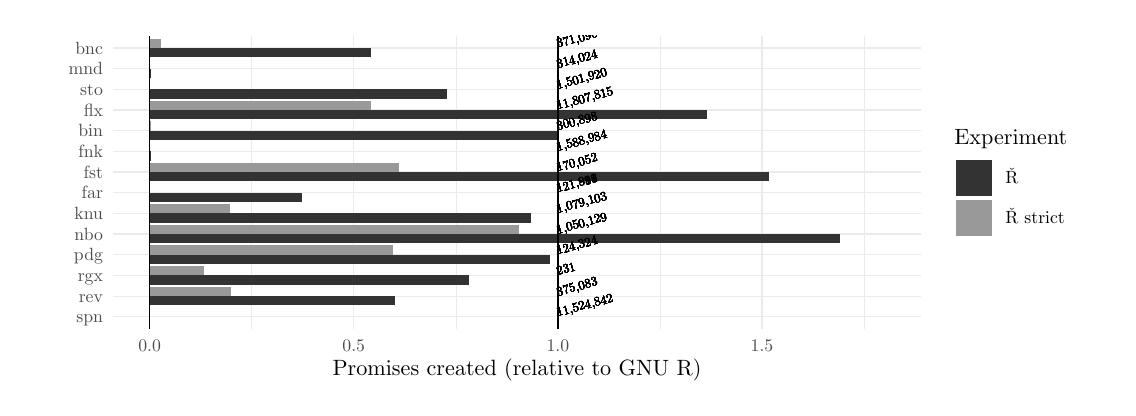
\begin{tikzpicture}[x=1pt,y=1pt]
\definecolor{fillColor}{RGB}{255,255,255}
\path[use as bounding box,fill=fillColor,fill opacity=0.00] (0,0) rectangle (390.26,130.09);
\begin{scope}
\path[clip] ( 30.80, 21.16) rectangle (322.87,127.24);
\definecolor{drawColor}{gray}{0.92}

\path[draw=drawColor,line width= 0.2pt,line join=round] ( 80.95, 21.16) --
	( 80.95,127.24);

\path[draw=drawColor,line width= 0.2pt,line join=round] (154.71, 21.16) --
	(154.71,127.24);

\path[draw=drawColor,line width= 0.2pt,line join=round] (228.46, 21.16) --
	(228.46,127.24);

\path[draw=drawColor,line width= 0.2pt,line join=round] (302.21, 21.16) --
	(302.21,127.24);

\path[draw=drawColor,line width= 0.4pt,line join=round] ( 30.80, 25.64) --
	(322.87, 25.64);

\path[draw=drawColor,line width= 0.4pt,line join=round] ( 30.80, 33.11) --
	(322.87, 33.11);

\path[draw=drawColor,line width= 0.4pt,line join=round] ( 30.80, 40.59) --
	(322.87, 40.59);

\path[draw=drawColor,line width= 0.4pt,line join=round] ( 30.80, 48.06) --
	(322.87, 48.06);

\path[draw=drawColor,line width= 0.4pt,line join=round] ( 30.80, 55.53) --
	(322.87, 55.53);

\path[draw=drawColor,line width= 0.4pt,line join=round] ( 30.80, 63.00) --
	(322.87, 63.00);

\path[draw=drawColor,line width= 0.4pt,line join=round] ( 30.80, 70.47) --
	(322.87, 70.47);

\path[draw=drawColor,line width= 0.4pt,line join=round] ( 30.80, 77.94) --
	(322.87, 77.94);

\path[draw=drawColor,line width= 0.4pt,line join=round] ( 30.80, 85.41) --
	(322.87, 85.41);

\path[draw=drawColor,line width= 0.4pt,line join=round] ( 30.80, 92.88) --
	(322.87, 92.88);

\path[draw=drawColor,line width= 0.4pt,line join=round] ( 30.80,100.35) --
	(322.87,100.35);

\path[draw=drawColor,line width= 0.4pt,line join=round] ( 30.80,107.82) --
	(322.87,107.82);

\path[draw=drawColor,line width= 0.4pt,line join=round] ( 30.80,115.29) --
	(322.87,115.29);

\path[draw=drawColor,line width= 0.4pt,line join=round] ( 30.80,122.76) --
	(322.87,122.76);

\path[draw=drawColor,line width= 0.4pt,line join=round] ( 44.07, 21.16) --
	( 44.07,127.24);

\path[draw=drawColor,line width= 0.4pt,line join=round] (117.83, 21.16) --
	(117.83,127.24);

\path[draw=drawColor,line width= 0.4pt,line join=round] (191.58, 21.16) --
	(191.58,127.24);

\path[draw=drawColor,line width= 0.4pt,line join=round] (265.34, 21.16) --
	(265.34,127.24);
\definecolor{fillColor}{gray}{0.60}

\path[fill=fillColor] ( 44.07,122.76) rectangle ( 48.25,126.12);

\path[fill=fillColor] ( 44.07,122.76) rectangle ( 48.25,126.12);

\path[fill=fillColor] ( 44.07,122.76) rectangle ( 48.25,126.12);

\path[fill=fillColor] ( 44.07,122.76) rectangle ( 48.25,126.12);

\path[fill=fillColor] ( 44.07,122.76) rectangle ( 48.25,126.12);

\path[fill=fillColor] ( 44.07,122.76) rectangle ( 48.25,126.12);

\path[fill=fillColor] ( 44.07,122.76) rectangle ( 48.25,126.12);

\path[fill=fillColor] ( 44.07,122.76) rectangle ( 48.25,126.12);

\path[fill=fillColor] ( 44.07,122.76) rectangle ( 48.25,126.12);

\path[fill=fillColor] ( 44.07,122.76) rectangle ( 48.25,126.12);
\definecolor{fillColor}{gray}{0.20}

\path[fill=fillColor] ( 44.07,119.40) rectangle (124.16,122.76);

\path[fill=fillColor] ( 44.07,119.40) rectangle (124.16,122.76);

\path[fill=fillColor] ( 44.07,119.40) rectangle (124.16,122.76);

\path[fill=fillColor] ( 44.07,119.40) rectangle (124.16,122.76);

\path[fill=fillColor] ( 44.07,119.40) rectangle (124.16,122.76);

\path[fill=fillColor] ( 44.07,119.40) rectangle (124.16,122.76);

\path[fill=fillColor] ( 44.07,119.40) rectangle (124.16,122.76);

\path[fill=fillColor] ( 44.07,119.40) rectangle (124.16,122.76);

\path[fill=fillColor] ( 44.07,119.40) rectangle (124.16,122.76);

\path[fill=fillColor] ( 44.07,119.40) rectangle (124.16,122.76);
\definecolor{fillColor}{gray}{0.60}

\path[fill=fillColor] ( 44.07,115.29) rectangle ( 44.07,118.65);

\path[fill=fillColor] ( 44.07,115.29) rectangle ( 44.07,118.65);

\path[fill=fillColor] ( 44.07,115.29) rectangle ( 44.07,118.65);

\path[fill=fillColor] ( 44.07,115.29) rectangle ( 44.07,118.65);

\path[fill=fillColor] ( 44.07,115.29) rectangle ( 44.07,118.65);

\path[fill=fillColor] ( 44.07,115.29) rectangle ( 44.07,118.65);

\path[fill=fillColor] ( 44.07,115.29) rectangle ( 44.07,118.65);

\path[fill=fillColor] ( 44.07,115.29) rectangle ( 44.07,118.65);

\path[fill=fillColor] ( 44.07,115.29) rectangle ( 44.07,118.65);

\path[fill=fillColor] ( 44.07,115.29) rectangle ( 44.07,118.65);
\definecolor{fillColor}{gray}{0.20}

\path[fill=fillColor] ( 44.07,111.93) rectangle ( 44.09,115.29);

\path[fill=fillColor] ( 44.07,111.93) rectangle ( 44.09,115.29);

\path[fill=fillColor] ( 44.07,111.93) rectangle ( 44.09,115.29);

\path[fill=fillColor] ( 44.07,111.93) rectangle ( 44.09,115.29);

\path[fill=fillColor] ( 44.07,111.93) rectangle ( 44.09,115.29);

\path[fill=fillColor] ( 44.07,111.93) rectangle ( 44.09,115.29);

\path[fill=fillColor] ( 44.07,111.93) rectangle ( 44.09,115.29);

\path[fill=fillColor] ( 44.07,111.93) rectangle ( 44.09,115.29);

\path[fill=fillColor] ( 44.07,111.93) rectangle ( 44.09,115.29);

\path[fill=fillColor] ( 44.07,111.93) rectangle ( 44.09,115.29);
\definecolor{fillColor}{gray}{0.60}

\path[fill=fillColor] ( 44.07,107.82) rectangle ( 44.07,111.18);

\path[fill=fillColor] ( 44.07,107.82) rectangle ( 44.07,111.18);

\path[fill=fillColor] ( 44.07,107.82) rectangle ( 44.07,111.18);

\path[fill=fillColor] ( 44.07,107.82) rectangle ( 44.07,111.18);

\path[fill=fillColor] ( 44.07,107.82) rectangle ( 44.07,111.18);

\path[fill=fillColor] ( 44.07,107.82) rectangle ( 44.07,111.18);

\path[fill=fillColor] ( 44.07,107.82) rectangle ( 44.07,111.18);

\path[fill=fillColor] ( 44.07,107.82) rectangle ( 44.07,111.18);

\path[fill=fillColor] ( 44.07,107.82) rectangle ( 44.07,111.18);

\path[fill=fillColor] ( 44.07,107.82) rectangle ( 44.07,111.18);
\definecolor{fillColor}{gray}{0.20}

\path[fill=fillColor] ( 44.07,104.46) rectangle (151.35,107.82);

\path[fill=fillColor] ( 44.07,104.46) rectangle (151.35,107.82);

\path[fill=fillColor] ( 44.07,104.46) rectangle (151.35,107.82);

\path[fill=fillColor] ( 44.07,104.46) rectangle (151.35,107.82);

\path[fill=fillColor] ( 44.07,104.46) rectangle (151.35,107.82);

\path[fill=fillColor] ( 44.07,104.46) rectangle (151.35,107.82);

\path[fill=fillColor] ( 44.07,104.46) rectangle (151.35,107.82);

\path[fill=fillColor] ( 44.07,104.46) rectangle (151.35,107.82);

\path[fill=fillColor] ( 44.07,104.46) rectangle (151.35,107.82);

\path[fill=fillColor] ( 44.07,104.46) rectangle (151.35,107.82);
\definecolor{fillColor}{gray}{0.60}

\path[fill=fillColor] ( 44.07,100.35) rectangle (124.05,103.71);

\path[fill=fillColor] ( 44.07,100.35) rectangle (124.05,103.71);

\path[fill=fillColor] ( 44.07,100.35) rectangle (124.05,103.71);

\path[fill=fillColor] ( 44.07,100.35) rectangle (124.05,103.71);

\path[fill=fillColor] ( 44.07,100.35) rectangle (124.05,103.71);

\path[fill=fillColor] ( 44.07,100.35) rectangle (124.05,103.71);

\path[fill=fillColor] ( 44.07,100.35) rectangle (124.05,103.71);

\path[fill=fillColor] ( 44.07,100.35) rectangle (124.05,103.71);

\path[fill=fillColor] ( 44.07,100.35) rectangle (124.05,103.71);

\path[fill=fillColor] ( 44.07,100.35) rectangle (124.05,103.71);
\definecolor{fillColor}{gray}{0.20}

\path[fill=fillColor] ( 44.07, 96.99) rectangle (245.34,100.35);

\path[fill=fillColor] ( 44.07, 96.99) rectangle (245.34,100.35);

\path[fill=fillColor] ( 44.07, 96.99) rectangle (245.34,100.35);

\path[fill=fillColor] ( 44.07, 96.99) rectangle (245.34,100.35);

\path[fill=fillColor] ( 44.07, 96.99) rectangle (245.34,100.35);

\path[fill=fillColor] ( 44.07, 96.99) rectangle (245.34,100.35);

\path[fill=fillColor] ( 44.07, 96.99) rectangle (245.34,100.35);

\path[fill=fillColor] ( 44.07, 96.99) rectangle (245.34,100.35);

\path[fill=fillColor] ( 44.07, 96.99) rectangle (245.34,100.35);

\path[fill=fillColor] ( 44.07, 96.99) rectangle (245.34,100.35);
\definecolor{fillColor}{gray}{0.60}

\path[fill=fillColor] ( 44.07, 92.88) rectangle ( 44.08, 96.24);

\path[fill=fillColor] ( 44.07, 92.88) rectangle ( 44.08, 96.24);

\path[fill=fillColor] ( 44.07, 92.88) rectangle ( 44.08, 96.24);

\path[fill=fillColor] ( 44.07, 92.88) rectangle ( 44.08, 96.24);

\path[fill=fillColor] ( 44.07, 92.88) rectangle ( 44.08, 96.24);

\path[fill=fillColor] ( 44.07, 92.88) rectangle ( 44.08, 96.24);

\path[fill=fillColor] ( 44.07, 92.88) rectangle ( 44.08, 96.24);

\path[fill=fillColor] ( 44.07, 92.88) rectangle ( 44.08, 96.24);

\path[fill=fillColor] ( 44.07, 92.88) rectangle ( 44.08, 96.24);

\path[fill=fillColor] ( 44.07, 92.88) rectangle ( 44.08, 96.24);
\definecolor{fillColor}{gray}{0.20}

\path[fill=fillColor] ( 44.07, 89.52) rectangle (191.57, 92.88);

\path[fill=fillColor] ( 44.07, 89.52) rectangle (191.57, 92.88);

\path[fill=fillColor] ( 44.07, 89.52) rectangle (191.57, 92.88);

\path[fill=fillColor] ( 44.07, 89.52) rectangle (191.57, 92.88);

\path[fill=fillColor] ( 44.07, 89.52) rectangle (191.57, 92.88);

\path[fill=fillColor] ( 44.07, 89.52) rectangle (191.57, 92.88);

\path[fill=fillColor] ( 44.07, 89.52) rectangle (191.57, 92.88);

\path[fill=fillColor] ( 44.07, 89.52) rectangle (191.57, 92.88);

\path[fill=fillColor] ( 44.07, 89.52) rectangle (191.57, 92.88);

\path[fill=fillColor] ( 44.07, 89.52) rectangle (191.57, 92.88);
\definecolor{fillColor}{gray}{0.60}

\path[fill=fillColor] ( 44.07, 85.41) rectangle ( 44.07, 88.77);

\path[fill=fillColor] ( 44.07, 85.41) rectangle ( 44.07, 88.77);

\path[fill=fillColor] ( 44.07, 85.41) rectangle ( 44.07, 88.77);

\path[fill=fillColor] ( 44.07, 85.41) rectangle ( 44.07, 88.77);

\path[fill=fillColor] ( 44.07, 85.41) rectangle ( 44.07, 88.77);

\path[fill=fillColor] ( 44.07, 85.41) rectangle ( 44.07, 88.77);

\path[fill=fillColor] ( 44.07, 85.41) rectangle ( 44.07, 88.77);

\path[fill=fillColor] ( 44.07, 85.41) rectangle ( 44.07, 88.77);

\path[fill=fillColor] ( 44.07, 85.41) rectangle ( 44.07, 88.77);

\path[fill=fillColor] ( 44.07, 85.41) rectangle ( 44.07, 88.77);
\definecolor{fillColor}{gray}{0.20}

\path[fill=fillColor] ( 44.07, 82.05) rectangle ( 44.08, 85.41);

\path[fill=fillColor] ( 44.07, 82.05) rectangle ( 44.08, 85.41);

\path[fill=fillColor] ( 44.07, 82.05) rectangle ( 44.08, 85.41);

\path[fill=fillColor] ( 44.07, 82.05) rectangle ( 44.08, 85.41);

\path[fill=fillColor] ( 44.07, 82.05) rectangle ( 44.08, 85.41);

\path[fill=fillColor] ( 44.07, 82.05) rectangle ( 44.08, 85.41);

\path[fill=fillColor] ( 44.07, 82.05) rectangle ( 44.08, 85.41);

\path[fill=fillColor] ( 44.07, 82.05) rectangle ( 44.08, 85.41);

\path[fill=fillColor] ( 44.07, 82.05) rectangle ( 44.08, 85.41);

\path[fill=fillColor] ( 44.07, 82.05) rectangle ( 44.08, 85.41);
\definecolor{fillColor}{gray}{0.60}

\path[fill=fillColor] ( 44.07, 77.94) rectangle (134.29, 81.30);

\path[fill=fillColor] ( 44.07, 77.94) rectangle (134.29, 81.30);

\path[fill=fillColor] ( 44.07, 77.94) rectangle (134.29, 81.30);

\path[fill=fillColor] ( 44.07, 77.94) rectangle (134.29, 81.30);

\path[fill=fillColor] ( 44.07, 77.94) rectangle (134.29, 81.30);

\path[fill=fillColor] ( 44.07, 77.94) rectangle (134.29, 81.30);

\path[fill=fillColor] ( 44.07, 77.94) rectangle (134.29, 81.30);

\path[fill=fillColor] ( 44.07, 77.94) rectangle (134.29, 81.30);

\path[fill=fillColor] ( 44.07, 77.94) rectangle (134.29, 81.30);

\path[fill=fillColor] ( 44.07, 77.94) rectangle (134.29, 81.30);
\definecolor{fillColor}{gray}{0.20}

\path[fill=fillColor] ( 44.07, 74.57) rectangle (267.90, 77.94);

\path[fill=fillColor] ( 44.07, 74.57) rectangle (267.90, 77.94);

\path[fill=fillColor] ( 44.07, 74.57) rectangle (267.90, 77.94);

\path[fill=fillColor] ( 44.07, 74.57) rectangle (267.90, 77.94);

\path[fill=fillColor] ( 44.07, 74.57) rectangle (267.90, 77.94);

\path[fill=fillColor] ( 44.07, 74.57) rectangle (267.90, 77.94);

\path[fill=fillColor] ( 44.07, 74.57) rectangle (267.90, 77.94);

\path[fill=fillColor] ( 44.07, 74.57) rectangle (267.90, 77.94);

\path[fill=fillColor] ( 44.07, 74.57) rectangle (267.90, 77.94);

\path[fill=fillColor] ( 44.07, 74.57) rectangle (267.90, 77.94);
\definecolor{fillColor}{gray}{0.60}

\path[fill=fillColor] ( 44.07, 70.47) rectangle ( 44.07, 73.83);

\path[fill=fillColor] ( 44.07, 70.47) rectangle ( 44.07, 73.83);

\path[fill=fillColor] ( 44.07, 70.47) rectangle ( 44.07, 73.83);

\path[fill=fillColor] ( 44.07, 70.47) rectangle ( 44.07, 73.83);

\path[fill=fillColor] ( 44.07, 70.47) rectangle ( 44.07, 73.83);

\path[fill=fillColor] ( 44.07, 70.47) rectangle ( 44.07, 73.83);

\path[fill=fillColor] ( 44.07, 70.47) rectangle ( 44.07, 73.83);

\path[fill=fillColor] ( 44.07, 70.47) rectangle ( 44.07, 73.83);

\path[fill=fillColor] ( 44.07, 70.47) rectangle ( 44.07, 73.83);

\path[fill=fillColor] ( 44.07, 70.47) rectangle ( 44.07, 73.83);
\definecolor{fillColor}{gray}{0.20}

\path[fill=fillColor] ( 44.07, 67.10) rectangle ( 98.96, 70.47);

\path[fill=fillColor] ( 44.07, 67.10) rectangle ( 98.96, 70.47);

\path[fill=fillColor] ( 44.07, 67.10) rectangle ( 98.96, 70.47);

\path[fill=fillColor] ( 44.07, 67.10) rectangle ( 98.96, 70.47);

\path[fill=fillColor] ( 44.07, 67.10) rectangle ( 98.96, 70.47);

\path[fill=fillColor] ( 44.07, 67.10) rectangle ( 98.96, 70.47);

\path[fill=fillColor] ( 44.07, 67.10) rectangle ( 98.96, 70.47);

\path[fill=fillColor] ( 44.07, 67.10) rectangle ( 98.96, 70.47);

\path[fill=fillColor] ( 44.07, 67.10) rectangle ( 98.96, 70.47);

\path[fill=fillColor] ( 44.07, 67.10) rectangle ( 98.96, 70.47);
\definecolor{fillColor}{gray}{0.60}

\path[fill=fillColor] ( 44.07, 63.00) rectangle ( 73.24, 66.36);

\path[fill=fillColor] ( 44.07, 63.00) rectangle ( 73.24, 66.36);

\path[fill=fillColor] ( 44.07, 63.00) rectangle ( 73.24, 66.36);

\path[fill=fillColor] ( 44.07, 63.00) rectangle ( 73.24, 66.36);

\path[fill=fillColor] ( 44.07, 63.00) rectangle ( 73.24, 66.36);

\path[fill=fillColor] ( 44.07, 63.00) rectangle ( 73.24, 66.36);

\path[fill=fillColor] ( 44.07, 63.00) rectangle ( 73.24, 66.36);

\path[fill=fillColor] ( 44.07, 63.00) rectangle ( 73.24, 66.36);

\path[fill=fillColor] ( 44.07, 63.00) rectangle ( 73.24, 66.36);

\path[fill=fillColor] ( 44.07, 63.00) rectangle ( 73.24, 66.36);
\definecolor{fillColor}{gray}{0.20}

\path[fill=fillColor] ( 44.07, 59.63) rectangle (181.99, 63.00);

\path[fill=fillColor] ( 44.07, 59.63) rectangle (181.99, 63.00);

\path[fill=fillColor] ( 44.07, 59.63) rectangle (181.99, 63.00);

\path[fill=fillColor] ( 44.07, 59.63) rectangle (181.99, 63.00);

\path[fill=fillColor] ( 44.07, 59.63) rectangle (181.99, 63.00);

\path[fill=fillColor] ( 44.07, 59.63) rectangle (181.99, 63.00);

\path[fill=fillColor] ( 44.07, 59.63) rectangle (181.99, 63.00);

\path[fill=fillColor] ( 44.07, 59.63) rectangle (181.99, 63.00);

\path[fill=fillColor] ( 44.07, 59.63) rectangle (181.99, 63.00);

\path[fill=fillColor] ( 44.07, 59.63) rectangle (181.99, 63.00);
\definecolor{fillColor}{gray}{0.60}

\path[fill=fillColor] ( 44.07, 55.53) rectangle (177.53, 58.89);

\path[fill=fillColor] ( 44.07, 55.53) rectangle (177.53, 58.89);

\path[fill=fillColor] ( 44.07, 55.53) rectangle (177.53, 58.89);

\path[fill=fillColor] ( 44.07, 55.53) rectangle (177.53, 58.89);

\path[fill=fillColor] ( 44.07, 55.53) rectangle (177.53, 58.89);

\path[fill=fillColor] ( 44.07, 55.53) rectangle (177.53, 58.89);

\path[fill=fillColor] ( 44.07, 55.53) rectangle (177.53, 58.89);

\path[fill=fillColor] ( 44.07, 55.53) rectangle (177.53, 58.89);

\path[fill=fillColor] ( 44.07, 55.53) rectangle (177.53, 58.89);

\path[fill=fillColor] ( 44.07, 55.53) rectangle (177.53, 58.89);
\definecolor{fillColor}{gray}{0.20}

\path[fill=fillColor] ( 44.07, 52.16) rectangle (293.42, 55.53);

\path[fill=fillColor] ( 44.07, 52.16) rectangle (293.42, 55.53);

\path[fill=fillColor] ( 44.07, 52.16) rectangle (293.42, 55.53);

\path[fill=fillColor] ( 44.07, 52.16) rectangle (293.42, 55.53);

\path[fill=fillColor] ( 44.07, 52.16) rectangle (293.42, 55.53);

\path[fill=fillColor] ( 44.07, 52.16) rectangle (293.42, 55.53);

\path[fill=fillColor] ( 44.07, 52.16) rectangle (293.42, 55.53);

\path[fill=fillColor] ( 44.07, 52.16) rectangle (293.42, 55.53);

\path[fill=fillColor] ( 44.07, 52.16) rectangle (293.42, 55.53);

\path[fill=fillColor] ( 44.07, 52.16) rectangle (293.42, 55.53);
\definecolor{fillColor}{gray}{0.60}

\path[fill=fillColor] ( 44.07, 48.06) rectangle (132.13, 51.42);

\path[fill=fillColor] ( 44.07, 48.06) rectangle (132.13, 51.42);

\path[fill=fillColor] ( 44.07, 48.06) rectangle (132.13, 51.42);

\path[fill=fillColor] ( 44.07, 48.06) rectangle (132.13, 51.42);

\path[fill=fillColor] ( 44.07, 48.06) rectangle (132.13, 51.42);

\path[fill=fillColor] ( 44.07, 48.06) rectangle (132.13, 51.42);

\path[fill=fillColor] ( 44.07, 48.06) rectangle (132.13, 51.42);

\path[fill=fillColor] ( 44.07, 48.06) rectangle (132.13, 51.42);

\path[fill=fillColor] ( 44.07, 48.06) rectangle (132.13, 51.42);

\path[fill=fillColor] ( 44.07, 48.06) rectangle (132.13, 51.42);
\definecolor{fillColor}{gray}{0.20}

\path[fill=fillColor] ( 44.07, 44.69) rectangle (188.90, 48.06);

\path[fill=fillColor] ( 44.07, 44.69) rectangle (188.90, 48.06);

\path[fill=fillColor] ( 44.07, 44.69) rectangle (188.90, 48.06);

\path[fill=fillColor] ( 44.07, 44.69) rectangle (188.90, 48.06);

\path[fill=fillColor] ( 44.07, 44.69) rectangle (188.90, 48.06);

\path[fill=fillColor] ( 44.07, 44.69) rectangle (188.90, 48.06);

\path[fill=fillColor] ( 44.07, 44.69) rectangle (188.90, 48.06);

\path[fill=fillColor] ( 44.07, 44.69) rectangle (188.90, 48.06);

\path[fill=fillColor] ( 44.07, 44.69) rectangle (188.90, 48.06);

\path[fill=fillColor] ( 44.07, 44.69) rectangle (188.90, 48.06);
\definecolor{fillColor}{gray}{0.60}

\path[fill=fillColor] ( 44.07, 40.59) rectangle ( 63.87, 43.95);

\path[fill=fillColor] ( 44.07, 40.59) rectangle ( 63.87, 43.95);

\path[fill=fillColor] ( 44.07, 40.59) rectangle ( 63.87, 43.95);

\path[fill=fillColor] ( 44.07, 40.59) rectangle ( 63.87, 43.95);

\path[fill=fillColor] ( 44.07, 40.59) rectangle ( 63.87, 43.95);

\path[fill=fillColor] ( 44.07, 40.59) rectangle ( 63.87, 43.95);

\path[fill=fillColor] ( 44.07, 40.59) rectangle ( 63.87, 43.95);

\path[fill=fillColor] ( 44.07, 40.59) rectangle ( 63.87, 43.95);

\path[fill=fillColor] ( 44.07, 40.59) rectangle ( 63.87, 43.95);

\path[fill=fillColor] ( 44.07, 40.59) rectangle ( 63.87, 43.95);
\definecolor{fillColor}{gray}{0.20}

\path[fill=fillColor] ( 44.07, 37.22) rectangle (159.65, 40.59);

\path[fill=fillColor] ( 44.07, 37.22) rectangle (159.65, 40.59);

\path[fill=fillColor] ( 44.07, 37.22) rectangle (159.65, 40.59);

\path[fill=fillColor] ( 44.07, 37.22) rectangle (159.65, 40.59);

\path[fill=fillColor] ( 44.07, 37.22) rectangle (159.65, 40.59);

\path[fill=fillColor] ( 44.07, 37.22) rectangle (159.65, 40.59);

\path[fill=fillColor] ( 44.07, 37.22) rectangle (159.65, 40.59);

\path[fill=fillColor] ( 44.07, 37.22) rectangle (159.65, 40.59);

\path[fill=fillColor] ( 44.07, 37.22) rectangle (159.65, 40.59);

\path[fill=fillColor] ( 44.07, 37.22) rectangle (159.65, 40.59);
\definecolor{fillColor}{gray}{0.60}

\path[fill=fillColor] ( 44.07, 33.11) rectangle ( 73.57, 36.48);

\path[fill=fillColor] ( 44.07, 33.11) rectangle ( 73.57, 36.48);

\path[fill=fillColor] ( 44.07, 33.11) rectangle ( 73.57, 36.48);

\path[fill=fillColor] ( 44.07, 33.11) rectangle ( 73.57, 36.48);

\path[fill=fillColor] ( 44.07, 33.11) rectangle ( 73.57, 36.48);

\path[fill=fillColor] ( 44.07, 33.11) rectangle ( 73.57, 36.48);

\path[fill=fillColor] ( 44.07, 33.11) rectangle ( 73.57, 36.48);

\path[fill=fillColor] ( 44.07, 33.11) rectangle ( 73.57, 36.48);

\path[fill=fillColor] ( 44.07, 33.11) rectangle ( 73.57, 36.48);

\path[fill=fillColor] ( 44.07, 33.11) rectangle ( 73.57, 36.48);
\definecolor{fillColor}{gray}{0.20}

\path[fill=fillColor] ( 44.07, 29.75) rectangle (132.58, 33.11);

\path[fill=fillColor] ( 44.07, 29.75) rectangle (132.58, 33.11);

\path[fill=fillColor] ( 44.07, 29.75) rectangle (132.58, 33.11);

\path[fill=fillColor] ( 44.07, 29.75) rectangle (132.58, 33.11);

\path[fill=fillColor] ( 44.07, 29.75) rectangle (132.58, 33.11);

\path[fill=fillColor] ( 44.07, 29.75) rectangle (132.58, 33.11);

\path[fill=fillColor] ( 44.07, 29.75) rectangle (132.58, 33.11);

\path[fill=fillColor] ( 44.07, 29.75) rectangle (132.58, 33.11);

\path[fill=fillColor] ( 44.07, 29.75) rectangle (132.58, 33.11);

\path[fill=fillColor] ( 44.07, 29.75) rectangle (132.58, 33.11);
\definecolor{fillColor}{gray}{0.60}

\path[fill=fillColor] ( 44.07, 25.64) rectangle ( 44.07, 29.01);

\path[fill=fillColor] ( 44.07, 25.64) rectangle ( 44.07, 29.01);

\path[fill=fillColor] ( 44.07, 25.64) rectangle ( 44.07, 29.01);

\path[fill=fillColor] ( 44.07, 25.64) rectangle ( 44.07, 29.01);

\path[fill=fillColor] ( 44.07, 25.64) rectangle ( 44.07, 29.01);

\path[fill=fillColor] ( 44.07, 25.64) rectangle ( 44.07, 29.01);

\path[fill=fillColor] ( 44.07, 25.64) rectangle ( 44.07, 29.01);

\path[fill=fillColor] ( 44.07, 25.64) rectangle ( 44.07, 29.01);

\path[fill=fillColor] ( 44.07, 25.64) rectangle ( 44.07, 29.01);

\path[fill=fillColor] ( 44.07, 25.64) rectangle ( 44.07, 29.01);
\definecolor{fillColor}{gray}{0.20}

\path[fill=fillColor] ( 44.07, 22.28) rectangle ( 44.07, 25.64);

\path[fill=fillColor] ( 44.07, 22.28) rectangle ( 44.07, 25.64);

\path[fill=fillColor] ( 44.07, 22.28) rectangle ( 44.07, 25.64);

\path[fill=fillColor] ( 44.07, 22.28) rectangle ( 44.07, 25.64);

\path[fill=fillColor] ( 44.07, 22.28) rectangle ( 44.07, 25.64);

\path[fill=fillColor] ( 44.07, 22.28) rectangle ( 44.07, 25.64);

\path[fill=fillColor] ( 44.07, 22.28) rectangle ( 44.07, 25.64);

\path[fill=fillColor] ( 44.07, 22.28) rectangle ( 44.07, 25.64);

\path[fill=fillColor] ( 44.07, 22.28) rectangle ( 44.07, 25.64);

\path[fill=fillColor] ( 44.07, 22.28) rectangle ( 44.07, 25.64);
\definecolor{drawColor}{RGB}{0,0,0}

\path[draw=drawColor,line width= 0.6pt,line join=round] ( 44.07, 21.16) -- ( 44.07,127.24);

\path[draw=drawColor,line width= 0.6pt,line join=round] (191.58, 21.16) -- (191.58,127.24);

\node[text=drawColor,rotate= 15.00,anchor=base west,inner sep=0pt, outer sep=0pt, scale=  0.46] at (191.58,122.76) {   371,090};

\node[text=drawColor,rotate= 15.00,anchor=base west,inner sep=0pt, outer sep=0pt, scale=  0.46] at (191.58,122.76) {   371,090};

\node[text=drawColor,rotate= 15.00,anchor=base west,inner sep=0pt, outer sep=0pt, scale=  0.46] at (191.58,122.76) {   371,090};

\node[text=drawColor,rotate= 15.00,anchor=base west,inner sep=0pt, outer sep=0pt, scale=  0.46] at (191.58,122.76) {   371,090};

\node[text=drawColor,rotate= 15.00,anchor=base west,inner sep=0pt, outer sep=0pt, scale=  0.46] at (191.58,122.76) {   371,090};

\node[text=drawColor,rotate= 15.00,anchor=base west,inner sep=0pt, outer sep=0pt, scale=  0.46] at (191.58,122.76) {   371,090};

\node[text=drawColor,rotate= 15.00,anchor=base west,inner sep=0pt, outer sep=0pt, scale=  0.46] at (191.58,122.76) {   371,090};

\node[text=drawColor,rotate= 15.00,anchor=base west,inner sep=0pt, outer sep=0pt, scale=  0.46] at (191.58,122.76) {   371,090};

\node[text=drawColor,rotate= 15.00,anchor=base west,inner sep=0pt, outer sep=0pt, scale=  0.46] at (191.58,122.76) {   371,090};

\node[text=drawColor,rotate= 15.00,anchor=base west,inner sep=0pt, outer sep=0pt, scale=  0.46] at (191.58,122.76) {   371,090};

\node[text=drawColor,rotate= 15.00,anchor=base west,inner sep=0pt, outer sep=0pt, scale=  0.46] at (191.58,115.29) {   314,024};

\node[text=drawColor,rotate= 15.00,anchor=base west,inner sep=0pt, outer sep=0pt, scale=  0.46] at (191.58,115.29) {   314,024};

\node[text=drawColor,rotate= 15.00,anchor=base west,inner sep=0pt, outer sep=0pt, scale=  0.46] at (191.58,115.29) {   314,024};

\node[text=drawColor,rotate= 15.00,anchor=base west,inner sep=0pt, outer sep=0pt, scale=  0.46] at (191.58,115.29) {   314,024};

\node[text=drawColor,rotate= 15.00,anchor=base west,inner sep=0pt, outer sep=0pt, scale=  0.46] at (191.58,115.29) {   314,024};

\node[text=drawColor,rotate= 15.00,anchor=base west,inner sep=0pt, outer sep=0pt, scale=  0.46] at (191.58,115.29) {   314,024};

\node[text=drawColor,rotate= 15.00,anchor=base west,inner sep=0pt, outer sep=0pt, scale=  0.46] at (191.58,115.29) {   314,024};

\node[text=drawColor,rotate= 15.00,anchor=base west,inner sep=0pt, outer sep=0pt, scale=  0.46] at (191.58,115.29) {   314,024};

\node[text=drawColor,rotate= 15.00,anchor=base west,inner sep=0pt, outer sep=0pt, scale=  0.46] at (191.58,115.29) {   314,024};

\node[text=drawColor,rotate= 15.00,anchor=base west,inner sep=0pt, outer sep=0pt, scale=  0.46] at (191.58,115.29) {   314,024};

\node[text=drawColor,rotate= 15.00,anchor=base west,inner sep=0pt, outer sep=0pt, scale=  0.46] at (191.58,107.82) { 1,501,920};

\node[text=drawColor,rotate= 15.00,anchor=base west,inner sep=0pt, outer sep=0pt, scale=  0.46] at (191.58,107.82) { 1,501,920};

\node[text=drawColor,rotate= 15.00,anchor=base west,inner sep=0pt, outer sep=0pt, scale=  0.46] at (191.58,107.82) { 1,501,920};

\node[text=drawColor,rotate= 15.00,anchor=base west,inner sep=0pt, outer sep=0pt, scale=  0.46] at (191.58,107.82) { 1,501,920};

\node[text=drawColor,rotate= 15.00,anchor=base west,inner sep=0pt, outer sep=0pt, scale=  0.46] at (191.58,107.82) { 1,501,920};

\node[text=drawColor,rotate= 15.00,anchor=base west,inner sep=0pt, outer sep=0pt, scale=  0.46] at (191.58,107.82) { 1,501,920};

\node[text=drawColor,rotate= 15.00,anchor=base west,inner sep=0pt, outer sep=0pt, scale=  0.46] at (191.58,107.82) { 1,501,920};

\node[text=drawColor,rotate= 15.00,anchor=base west,inner sep=0pt, outer sep=0pt, scale=  0.46] at (191.58,107.82) { 1,501,920};

\node[text=drawColor,rotate= 15.00,anchor=base west,inner sep=0pt, outer sep=0pt, scale=  0.46] at (191.58,107.82) { 1,501,920};

\node[text=drawColor,rotate= 15.00,anchor=base west,inner sep=0pt, outer sep=0pt, scale=  0.46] at (191.58,107.82) { 1,501,920};

\node[text=drawColor,rotate= 15.00,anchor=base west,inner sep=0pt, outer sep=0pt, scale=  0.46] at (191.58,100.35) {11,807,815};

\node[text=drawColor,rotate= 15.00,anchor=base west,inner sep=0pt, outer sep=0pt, scale=  0.46] at (191.58,100.35) {11,807,815};

\node[text=drawColor,rotate= 15.00,anchor=base west,inner sep=0pt, outer sep=0pt, scale=  0.46] at (191.58,100.35) {11,807,815};

\node[text=drawColor,rotate= 15.00,anchor=base west,inner sep=0pt, outer sep=0pt, scale=  0.46] at (191.58,100.35) {11,807,815};

\node[text=drawColor,rotate= 15.00,anchor=base west,inner sep=0pt, outer sep=0pt, scale=  0.46] at (191.58,100.35) {11,807,815};

\node[text=drawColor,rotate= 15.00,anchor=base west,inner sep=0pt, outer sep=0pt, scale=  0.46] at (191.58,100.35) {11,807,815};

\node[text=drawColor,rotate= 15.00,anchor=base west,inner sep=0pt, outer sep=0pt, scale=  0.46] at (191.58,100.35) {11,807,815};

\node[text=drawColor,rotate= 15.00,anchor=base west,inner sep=0pt, outer sep=0pt, scale=  0.46] at (191.58,100.35) {11,807,815};

\node[text=drawColor,rotate= 15.00,anchor=base west,inner sep=0pt, outer sep=0pt, scale=  0.46] at (191.58,100.35) {11,807,815};

\node[text=drawColor,rotate= 15.00,anchor=base west,inner sep=0pt, outer sep=0pt, scale=  0.46] at (191.58,100.35) {11,807,815};

\node[text=drawColor,rotate= 15.00,anchor=base west,inner sep=0pt, outer sep=0pt, scale=  0.46] at (191.58, 92.88) {   300,898};

\node[text=drawColor,rotate= 15.00,anchor=base west,inner sep=0pt, outer sep=0pt, scale=  0.46] at (191.58, 92.88) {   300,898};

\node[text=drawColor,rotate= 15.00,anchor=base west,inner sep=0pt, outer sep=0pt, scale=  0.46] at (191.58, 92.88) {   300,898};

\node[text=drawColor,rotate= 15.00,anchor=base west,inner sep=0pt, outer sep=0pt, scale=  0.46] at (191.58, 92.88) {   300,898};

\node[text=drawColor,rotate= 15.00,anchor=base west,inner sep=0pt, outer sep=0pt, scale=  0.46] at (191.58, 92.88) {   300,898};

\node[text=drawColor,rotate= 15.00,anchor=base west,inner sep=0pt, outer sep=0pt, scale=  0.46] at (191.58, 92.88) {   300,898};

\node[text=drawColor,rotate= 15.00,anchor=base west,inner sep=0pt, outer sep=0pt, scale=  0.46] at (191.58, 92.88) {   300,898};

\node[text=drawColor,rotate= 15.00,anchor=base west,inner sep=0pt, outer sep=0pt, scale=  0.46] at (191.58, 92.88) {   300,898};

\node[text=drawColor,rotate= 15.00,anchor=base west,inner sep=0pt, outer sep=0pt, scale=  0.46] at (191.58, 92.88) {   300,898};

\node[text=drawColor,rotate= 15.00,anchor=base west,inner sep=0pt, outer sep=0pt, scale=  0.46] at (191.58, 92.88) {   300,898};

\node[text=drawColor,rotate= 15.00,anchor=base west,inner sep=0pt, outer sep=0pt, scale=  0.46] at (191.58, 85.41) { 1,588,984};

\node[text=drawColor,rotate= 15.00,anchor=base west,inner sep=0pt, outer sep=0pt, scale=  0.46] at (191.58, 85.41) { 1,588,984};

\node[text=drawColor,rotate= 15.00,anchor=base west,inner sep=0pt, outer sep=0pt, scale=  0.46] at (191.58, 85.41) { 1,588,984};

\node[text=drawColor,rotate= 15.00,anchor=base west,inner sep=0pt, outer sep=0pt, scale=  0.46] at (191.58, 85.41) { 1,588,984};

\node[text=drawColor,rotate= 15.00,anchor=base west,inner sep=0pt, outer sep=0pt, scale=  0.46] at (191.58, 85.41) { 1,588,984};

\node[text=drawColor,rotate= 15.00,anchor=base west,inner sep=0pt, outer sep=0pt, scale=  0.46] at (191.58, 85.41) { 1,588,984};

\node[text=drawColor,rotate= 15.00,anchor=base west,inner sep=0pt, outer sep=0pt, scale=  0.46] at (191.58, 85.41) { 1,588,984};

\node[text=drawColor,rotate= 15.00,anchor=base west,inner sep=0pt, outer sep=0pt, scale=  0.46] at (191.58, 85.41) { 1,588,984};

\node[text=drawColor,rotate= 15.00,anchor=base west,inner sep=0pt, outer sep=0pt, scale=  0.46] at (191.58, 85.41) { 1,588,984};

\node[text=drawColor,rotate= 15.00,anchor=base west,inner sep=0pt, outer sep=0pt, scale=  0.46] at (191.58, 85.41) { 1,588,984};

\node[text=drawColor,rotate= 15.00,anchor=base west,inner sep=0pt, outer sep=0pt, scale=  0.46] at (191.58, 77.94) {   170,052};

\node[text=drawColor,rotate= 15.00,anchor=base west,inner sep=0pt, outer sep=0pt, scale=  0.46] at (191.58, 77.94) {   170,052};

\node[text=drawColor,rotate= 15.00,anchor=base west,inner sep=0pt, outer sep=0pt, scale=  0.46] at (191.58, 77.94) {   170,052};

\node[text=drawColor,rotate= 15.00,anchor=base west,inner sep=0pt, outer sep=0pt, scale=  0.46] at (191.58, 77.94) {   170,052};

\node[text=drawColor,rotate= 15.00,anchor=base west,inner sep=0pt, outer sep=0pt, scale=  0.46] at (191.58, 77.94) {   170,052};

\node[text=drawColor,rotate= 15.00,anchor=base west,inner sep=0pt, outer sep=0pt, scale=  0.46] at (191.58, 77.94) {   170,052};

\node[text=drawColor,rotate= 15.00,anchor=base west,inner sep=0pt, outer sep=0pt, scale=  0.46] at (191.58, 77.94) {   170,052};

\node[text=drawColor,rotate= 15.00,anchor=base west,inner sep=0pt, outer sep=0pt, scale=  0.46] at (191.58, 77.94) {   170,052};

\node[text=drawColor,rotate= 15.00,anchor=base west,inner sep=0pt, outer sep=0pt, scale=  0.46] at (191.58, 77.94) {   170,052};

\node[text=drawColor,rotate= 15.00,anchor=base west,inner sep=0pt, outer sep=0pt, scale=  0.46] at (191.58, 77.94) {   170,052};

\node[text=drawColor,rotate= 15.00,anchor=base west,inner sep=0pt, outer sep=0pt, scale=  0.46] at (191.58, 70.47) {   121,882};

\node[text=drawColor,rotate= 15.00,anchor=base west,inner sep=0pt, outer sep=0pt, scale=  0.46] at (191.58, 70.47) {   121,891};

\node[text=drawColor,rotate= 15.00,anchor=base west,inner sep=0pt, outer sep=0pt, scale=  0.46] at (191.58, 70.47) {   121,891};

\node[text=drawColor,rotate= 15.00,anchor=base west,inner sep=0pt, outer sep=0pt, scale=  0.46] at (191.58, 70.47) {   121,891};

\node[text=drawColor,rotate= 15.00,anchor=base west,inner sep=0pt, outer sep=0pt, scale=  0.46] at (191.58, 70.47) {   121,918};

\node[text=drawColor,rotate= 15.00,anchor=base west,inner sep=0pt, outer sep=0pt, scale=  0.46] at (191.58, 70.47) {   121,918};

\node[text=drawColor,rotate= 15.00,anchor=base west,inner sep=0pt, outer sep=0pt, scale=  0.46] at (191.58, 70.47) {   121,921};

\node[text=drawColor,rotate= 15.00,anchor=base west,inner sep=0pt, outer sep=0pt, scale=  0.46] at (191.58, 70.47) {   121,936};

\node[text=drawColor,rotate= 15.00,anchor=base west,inner sep=0pt, outer sep=0pt, scale=  0.46] at (191.58, 70.47) {   121,957};

\node[text=drawColor,rotate= 15.00,anchor=base west,inner sep=0pt, outer sep=0pt, scale=  0.46] at (191.58, 70.47) {   121,969};

\node[text=drawColor,rotate= 15.00,anchor=base west,inner sep=0pt, outer sep=0pt, scale=  0.46] at (191.58, 63.00) { 1,079,103};

\node[text=drawColor,rotate= 15.00,anchor=base west,inner sep=0pt, outer sep=0pt, scale=  0.46] at (191.58, 63.00) { 1,079,103};

\node[text=drawColor,rotate= 15.00,anchor=base west,inner sep=0pt, outer sep=0pt, scale=  0.46] at (191.58, 63.00) { 1,079,103};

\node[text=drawColor,rotate= 15.00,anchor=base west,inner sep=0pt, outer sep=0pt, scale=  0.46] at (191.58, 63.00) { 1,079,103};

\node[text=drawColor,rotate= 15.00,anchor=base west,inner sep=0pt, outer sep=0pt, scale=  0.46] at (191.58, 63.00) { 1,079,103};

\node[text=drawColor,rotate= 15.00,anchor=base west,inner sep=0pt, outer sep=0pt, scale=  0.46] at (191.58, 63.00) { 1,079,103};

\node[text=drawColor,rotate= 15.00,anchor=base west,inner sep=0pt, outer sep=0pt, scale=  0.46] at (191.58, 63.00) { 1,079,103};

\node[text=drawColor,rotate= 15.00,anchor=base west,inner sep=0pt, outer sep=0pt, scale=  0.46] at (191.58, 63.00) { 1,079,103};

\node[text=drawColor,rotate= 15.00,anchor=base west,inner sep=0pt, outer sep=0pt, scale=  0.46] at (191.58, 63.00) { 1,079,103};

\node[text=drawColor,rotate= 15.00,anchor=base west,inner sep=0pt, outer sep=0pt, scale=  0.46] at (191.58, 63.00) { 1,079,103};

\node[text=drawColor,rotate= 15.00,anchor=base west,inner sep=0pt, outer sep=0pt, scale=  0.46] at (191.58, 55.53) { 1,050,129};

\node[text=drawColor,rotate= 15.00,anchor=base west,inner sep=0pt, outer sep=0pt, scale=  0.46] at (191.58, 55.53) { 1,050,129};

\node[text=drawColor,rotate= 15.00,anchor=base west,inner sep=0pt, outer sep=0pt, scale=  0.46] at (191.58, 55.53) { 1,050,129};

\node[text=drawColor,rotate= 15.00,anchor=base west,inner sep=0pt, outer sep=0pt, scale=  0.46] at (191.58, 55.53) { 1,050,129};

\node[text=drawColor,rotate= 15.00,anchor=base west,inner sep=0pt, outer sep=0pt, scale=  0.46] at (191.58, 55.53) { 1,050,129};

\node[text=drawColor,rotate= 15.00,anchor=base west,inner sep=0pt, outer sep=0pt, scale=  0.46] at (191.58, 55.53) { 1,050,129};

\node[text=drawColor,rotate= 15.00,anchor=base west,inner sep=0pt, outer sep=0pt, scale=  0.46] at (191.58, 55.53) { 1,050,129};

\node[text=drawColor,rotate= 15.00,anchor=base west,inner sep=0pt, outer sep=0pt, scale=  0.46] at (191.58, 55.53) { 1,050,129};

\node[text=drawColor,rotate= 15.00,anchor=base west,inner sep=0pt, outer sep=0pt, scale=  0.46] at (191.58, 55.53) { 1,050,129};

\node[text=drawColor,rotate= 15.00,anchor=base west,inner sep=0pt, outer sep=0pt, scale=  0.46] at (191.58, 55.53) { 1,050,129};

\node[text=drawColor,rotate= 15.00,anchor=base west,inner sep=0pt, outer sep=0pt, scale=  0.46] at (191.58, 48.06) {   124,324};

\node[text=drawColor,rotate= 15.00,anchor=base west,inner sep=0pt, outer sep=0pt, scale=  0.46] at (191.58, 48.06) {   124,324};

\node[text=drawColor,rotate= 15.00,anchor=base west,inner sep=0pt, outer sep=0pt, scale=  0.46] at (191.58, 48.06) {   124,324};

\node[text=drawColor,rotate= 15.00,anchor=base west,inner sep=0pt, outer sep=0pt, scale=  0.46] at (191.58, 48.06) {   124,324};

\node[text=drawColor,rotate= 15.00,anchor=base west,inner sep=0pt, outer sep=0pt, scale=  0.46] at (191.58, 48.06) {   124,324};

\node[text=drawColor,rotate= 15.00,anchor=base west,inner sep=0pt, outer sep=0pt, scale=  0.46] at (191.58, 48.06) {   124,324};

\node[text=drawColor,rotate= 15.00,anchor=base west,inner sep=0pt, outer sep=0pt, scale=  0.46] at (191.58, 48.06) {   124,324};

\node[text=drawColor,rotate= 15.00,anchor=base west,inner sep=0pt, outer sep=0pt, scale=  0.46] at (191.58, 48.06) {   124,324};

\node[text=drawColor,rotate= 15.00,anchor=base west,inner sep=0pt, outer sep=0pt, scale=  0.46] at (191.58, 48.06) {   124,324};

\node[text=drawColor,rotate= 15.00,anchor=base west,inner sep=0pt, outer sep=0pt, scale=  0.46] at (191.58, 48.06) {   124,324};

\node[text=drawColor,rotate= 15.00,anchor=base west,inner sep=0pt, outer sep=0pt, scale=  0.46] at (191.58, 40.59) {       231};

\node[text=drawColor,rotate= 15.00,anchor=base west,inner sep=0pt, outer sep=0pt, scale=  0.46] at (191.58, 40.59) {       231};

\node[text=drawColor,rotate= 15.00,anchor=base west,inner sep=0pt, outer sep=0pt, scale=  0.46] at (191.58, 40.59) {       231};

\node[text=drawColor,rotate= 15.00,anchor=base west,inner sep=0pt, outer sep=0pt, scale=  0.46] at (191.58, 40.59) {       231};

\node[text=drawColor,rotate= 15.00,anchor=base west,inner sep=0pt, outer sep=0pt, scale=  0.46] at (191.58, 40.59) {       231};

\node[text=drawColor,rotate= 15.00,anchor=base west,inner sep=0pt, outer sep=0pt, scale=  0.46] at (191.58, 40.59) {       231};

\node[text=drawColor,rotate= 15.00,anchor=base west,inner sep=0pt, outer sep=0pt, scale=  0.46] at (191.58, 40.59) {       231};

\node[text=drawColor,rotate= 15.00,anchor=base west,inner sep=0pt, outer sep=0pt, scale=  0.46] at (191.58, 40.59) {       231};

\node[text=drawColor,rotate= 15.00,anchor=base west,inner sep=0pt, outer sep=0pt, scale=  0.46] at (191.58, 40.59) {       231};

\node[text=drawColor,rotate= 15.00,anchor=base west,inner sep=0pt, outer sep=0pt, scale=  0.46] at (191.58, 40.59) {       231};

\node[text=drawColor,rotate= 15.00,anchor=base west,inner sep=0pt, outer sep=0pt, scale=  0.46] at (191.58, 33.11) {   375,083};

\node[text=drawColor,rotate= 15.00,anchor=base west,inner sep=0pt, outer sep=0pt, scale=  0.46] at (191.58, 33.11) {   375,083};

\node[text=drawColor,rotate= 15.00,anchor=base west,inner sep=0pt, outer sep=0pt, scale=  0.46] at (191.58, 33.11) {   375,083};

\node[text=drawColor,rotate= 15.00,anchor=base west,inner sep=0pt, outer sep=0pt, scale=  0.46] at (191.58, 33.11) {   375,083};

\node[text=drawColor,rotate= 15.00,anchor=base west,inner sep=0pt, outer sep=0pt, scale=  0.46] at (191.58, 33.11) {   375,083};

\node[text=drawColor,rotate= 15.00,anchor=base west,inner sep=0pt, outer sep=0pt, scale=  0.46] at (191.58, 33.11) {   375,083};

\node[text=drawColor,rotate= 15.00,anchor=base west,inner sep=0pt, outer sep=0pt, scale=  0.46] at (191.58, 33.11) {   375,083};

\node[text=drawColor,rotate= 15.00,anchor=base west,inner sep=0pt, outer sep=0pt, scale=  0.46] at (191.58, 33.11) {   375,083};

\node[text=drawColor,rotate= 15.00,anchor=base west,inner sep=0pt, outer sep=0pt, scale=  0.46] at (191.58, 33.11) {   375,083};

\node[text=drawColor,rotate= 15.00,anchor=base west,inner sep=0pt, outer sep=0pt, scale=  0.46] at (191.58, 33.11) {   375,083};

\node[text=drawColor,rotate= 15.00,anchor=base west,inner sep=0pt, outer sep=0pt, scale=  0.46] at (191.58, 25.64) {11,524,842};

\node[text=drawColor,rotate= 15.00,anchor=base west,inner sep=0pt, outer sep=0pt, scale=  0.46] at (191.58, 25.64) {11,524,842};

\node[text=drawColor,rotate= 15.00,anchor=base west,inner sep=0pt, outer sep=0pt, scale=  0.46] at (191.58, 25.64) {11,524,842};

\node[text=drawColor,rotate= 15.00,anchor=base west,inner sep=0pt, outer sep=0pt, scale=  0.46] at (191.58, 25.64) {11,524,842};

\node[text=drawColor,rotate= 15.00,anchor=base west,inner sep=0pt, outer sep=0pt, scale=  0.46] at (191.58, 25.64) {11,524,842};

\node[text=drawColor,rotate= 15.00,anchor=base west,inner sep=0pt, outer sep=0pt, scale=  0.46] at (191.58, 25.64) {11,524,842};

\node[text=drawColor,rotate= 15.00,anchor=base west,inner sep=0pt, outer sep=0pt, scale=  0.46] at (191.58, 25.64) {11,524,842};

\node[text=drawColor,rotate= 15.00,anchor=base west,inner sep=0pt, outer sep=0pt, scale=  0.46] at (191.58, 25.64) {11,524,842};

\node[text=drawColor,rotate= 15.00,anchor=base west,inner sep=0pt, outer sep=0pt, scale=  0.46] at (191.58, 25.64) {11,524,842};

\node[text=drawColor,rotate= 15.00,anchor=base west,inner sep=0pt, outer sep=0pt, scale=  0.46] at (191.58, 25.64) {11,524,842};
\end{scope}
\begin{scope}
\path[clip] (  0.00,  0.00) rectangle (390.26,130.09);
\definecolor{drawColor}{gray}{0.30}

\node[text=drawColor,anchor=base east,inner sep=0pt, outer sep=0pt, scale=  0.64] at ( 27.20, 23.44) {spn};

\node[text=drawColor,anchor=base east,inner sep=0pt, outer sep=0pt, scale=  0.64] at ( 27.20, 30.91) {rev};

\node[text=drawColor,anchor=base east,inner sep=0pt, outer sep=0pt, scale=  0.64] at ( 27.20, 38.38) {rgx};

\node[text=drawColor,anchor=base east,inner sep=0pt, outer sep=0pt, scale=  0.64] at ( 27.20, 45.85) {pdg};

\node[text=drawColor,anchor=base east,inner sep=0pt, outer sep=0pt, scale=  0.64] at ( 27.20, 53.32) {nbo};

\node[text=drawColor,anchor=base east,inner sep=0pt, outer sep=0pt, scale=  0.64] at ( 27.20, 60.79) {knu};

\node[text=drawColor,anchor=base east,inner sep=0pt, outer sep=0pt, scale=  0.64] at ( 27.20, 68.26) {far};

\node[text=drawColor,anchor=base east,inner sep=0pt, outer sep=0pt, scale=  0.64] at ( 27.20, 75.73) {fst};

\node[text=drawColor,anchor=base east,inner sep=0pt, outer sep=0pt, scale=  0.64] at ( 27.20, 83.20) {fnk};

\node[text=drawColor,anchor=base east,inner sep=0pt, outer sep=0pt, scale=  0.64] at ( 27.20, 90.67) {bin};

\node[text=drawColor,anchor=base east,inner sep=0pt, outer sep=0pt, scale=  0.64] at ( 27.20, 98.14) {flx};

\node[text=drawColor,anchor=base east,inner sep=0pt, outer sep=0pt, scale=  0.64] at ( 27.20,105.61) {sto};

\node[text=drawColor,anchor=base east,inner sep=0pt, outer sep=0pt, scale=  0.64] at ( 27.20,113.08) {mnd};

\node[text=drawColor,anchor=base east,inner sep=0pt, outer sep=0pt, scale=  0.64] at ( 27.20,120.55) {bnc};
\end{scope}
\begin{scope}
\path[clip] (  0.00,  0.00) rectangle (390.26,130.09);
\definecolor{drawColor}{gray}{0.30}

\node[text=drawColor,anchor=base,inner sep=0pt, outer sep=0pt, scale=  0.64] at ( 44.07, 13.15) {0.0};

\node[text=drawColor,anchor=base,inner sep=0pt, outer sep=0pt, scale=  0.64] at (117.83, 13.15) {0.5};

\node[text=drawColor,anchor=base,inner sep=0pt, outer sep=0pt, scale=  0.64] at (191.58, 13.15) {1.0};

\node[text=drawColor,anchor=base,inner sep=0pt, outer sep=0pt, scale=  0.64] at (265.34, 13.15) {1.5};
\end{scope}
\begin{scope}
\path[clip] (  0.00,  0.00) rectangle (390.26,130.09);
\definecolor{drawColor}{RGB}{0,0,0}

\node[text=drawColor,anchor=base,inner sep=0pt, outer sep=0pt, scale=  0.80] at (176.83,  4.40) {Promises created (relative to GNU R)};
\end{scope}
\begin{scope}
\path[clip] (  0.00,  0.00) rectangle (390.26,130.09);
\definecolor{drawColor}{RGB}{0,0,0}

\node[text=drawColor,anchor=base west,inner sep=0pt, outer sep=0pt, scale=  0.80] at (334.87, 87.90) {Experiment};
\end{scope}
\begin{scope}
\path[clip] (  0.00,  0.00) rectangle (390.26,130.09);
\definecolor{fillColor}{gray}{0.20}

\path[fill=fillColor] (335.58, 69.38) rectangle (348.61, 82.41);
\end{scope}
\begin{scope}
\path[clip] (  0.00,  0.00) rectangle (390.26,130.09);
\definecolor{fillColor}{gray}{0.60}

\path[fill=fillColor] (335.58, 54.93) rectangle (348.61, 67.96);
\end{scope}
\begin{scope}
\path[clip] (  0.00,  0.00) rectangle (390.26,130.09);
\definecolor{drawColor}{RGB}{0,0,0}

\node[text=drawColor,anchor=base west,inner sep=0pt, outer sep=0pt, scale=  0.64] at (353.32, 73.69) {\v{R}};
\end{scope}
\begin{scope}
\path[clip] (  0.00,  0.00) rectangle (390.26,130.09);
\definecolor{drawColor}{RGB}{0,0,0}

\node[text=drawColor,anchor=base west,inner sep=0pt, outer sep=0pt, scale=  0.64] at (353.32, 59.24) {\v{R} strict};
\end{scope}
\end{tikzpicture}

  \caption{Promises allocated, normalized to GNU R. The right column shows GNU R's actual promises. If the bar is too small to display, we show the actual number of promises in the respective experiment.}
  \label{fig:gc-pressure}
\end{figure}

We measure the number of promises allocated in the benchmark suite per iteration
for GNU R, \Rsh, and \rshstrict. The results are shown in
\autoref{fig:gc-pressure}. We report on the geometric mean of the reductions in
each benchmark.

The first jump from GNU R's bytecode interpreter to the optimizing just-in-time
compiler \Rsh, leads to a \promiseAlocationReductionGnurRsh reduction in
allocations. The number is reached by taking the geometric mean of light-gray
bars, yielding a \promiseAllocationGnurRsh. Therefore, the reduction is
\promiseAlocationReductionGnurRsh ({$100\%$\xspace} -
\promiseAllocationGnurRsh). Note that for some benchmarks the light-gray bar is
too small to be seen and replaced by the actual number.

The second step from lazy to eager semantics leads to
\promiseAlocationReductionRshStrictToZero benchmarks not allocating any promises
at all. On the remainder, we see an additional
\promiseAlocationReductionRshStrict reduction (\rshstrict normalized to \Rsh).

Overall, \promiseAlocationReductionRshStrictToZero benchmarks reduce to zero
allocations, the rest reduce on average by
\promiseAlocationReductionGnurRshStrict. To reach this number, once again we
compute the geometric mean of dark bars, yielding
\promiseAllocatioGnurRshStrict. Therefore, the reduction is
~\promiseAlocationReductionGnurRshStrict ({$100\%$\xspace} -
\promiseAllocatioGnurRshStrict).

The lowest reduction observed is \promiseAlocationReductionGnurRshStrictMin.
Surprisingly the number of remaining promises is still relatively high in some
cases. As far as we were able to observe, they originate largely from special
forms, \ie R builtins with a custom evaluation strategy, that are not yet
natively supported in the \Rsh bytecode.

It turns out that even an optimizing compiler has to allocate many promises for
R code, as oftentimes, they cannot be eliminated entirely. \rshstrict allows for
a larger reduction in the number of promises allocated. Thus, we expected a
significant portion of the overall speedup to originate from the reduced
allocation rate. We measured the differences in garbage collection time and it
ranged from \speedupGCRshStrictMin to \speedupGCRshStrictMax, but found the
contribution to the overall speedup to be smaller than expected. The GNU R
garbage collector, which is reused in \Rsh, has a fairly slow allocation path,
which includes mutating a doubly-linked list. Therefore, some portion of the
speedup could be due to the saved time in the allocation of promises, which is
not counted in the GC time. We therefore conducted an additional experiment,
where we evaluated arguments to calls eagerly, but additionally allocated a
promise only to be subsequently discarded. This configuration led to an overall
speedup of \speedupBCRshStrictAlloc instead of \speedupBCRshStrict, suggesting
that about \speedupDueToReducedGC of the performance improvement in the bytecode
interpreter is due to the reduced allocation. Unfortunately, a similar
experiment cannot be as easily conducted for the optimizing tier of \Rsh, since
its compiler would just optimize away all unnecessary allocations. We conjecture
that the contribution should be even smaller in that case, because it allocates
much fewer promises to start with.

\paragraph{Discussion}

In both tiers, we observed a proportional reduction of time spent tracing the
heap and allocating promises. Surprisingly, that was not the main reason
for the speedups. We investigated the remaining difference using the
\lstinline{perf} profiler and found that the overheads of lazy evaluation are to
be found in setting up the execution context for promise evaluation. This
includes marking it as 'executing' to detect recursive evaluation dependencies,
and either calling the interpreter's main eval-loop on the code of the promise or
calling the compiled function. In the case of the native backend, having the
promises inlined at the call-site instead of in a separate native function
invoked by the callee, resulted in fewer instruction cache misses. We also found
some instances where both tiers sped up similarly, however, the underlying
reasons were very different. Take for instance the \lstinline{bin} benchmark,
which showed in both interpreter and compiler a speedup of about $1.5\times$ in
the strict mode. In native, the execution time decreased from 79ms to 53ms. In
the interpreter, time went from 143ms to 97ms per iteration. In the former case,
the speedup comes from the effects described above; for the latter, part of the
speedup is due to better optimizations. Previously the local environment of
the innermost function was live. Thanks to eager evaluation of the arguments,
the argument promises do not leak the environment and therefore \Rsh is able to
elide it.

\section{Conclusion}\label{sec:conclusion}

In R, function arguments are not evaluated at the call-site, instead, the
evaluation is suspended until the callee needs it. The definition of
\emph{need} is quite liberal here as, for example, local re-binding, returning,
and many builtin functions are strict. As was reported in previous work, this
leads to many programs being on the eager side of the spectrum for a lazy
language. Why is R lazy at all? It turns out that allowing users to reflectively
alter argument expressions, before evaluating them, is a very expressive and
powerful meta-programming technique, enjoyed by many package authors in the R
ecosystem to build, \eg embedded domain specific languages. It is part of
what makes R appealing to its users, even if they do not realize that the
language they use has a lazy core. However, the joy is limited when it comes to
writing robust R code --- as both the caller and the callee co-determine what a function
actually does --- and also when implementing the language itself. When we turned
R into a mostly strict mode, the \Rsh just-in-time compiler ran
\speedupRshStrict faster through our benchmarks without any further changes.
Taking everything into account, we believe that R should be strict by default,
giving package authors the option to opt-in to laziness. We provide a strategy
for R as an ecosystem to get there by automatically inferring robust strictness
signatures for package code. These signatures try to capture the desired and
accidental laziness of arguments passed to R packages, thereby allowing most of
the client code to run unchanged --- in our experiments, only \robustnesResult of
all depending packages' tests failed. Such automatically generated strictness
signatures can then subsequently be refined by the package authors and users.
The change to the language would be beneficial in several ways. Implementations
would become faster, compilers and program analysis easier to perform, users
would be presented with a more commonly expected call semantic, and it would open
up the path for further evolution. Currently, many standard techniques such as
gradually typed function signatures and efficient just-in-time optimizations are
difficult to apply to R because of laziness.

\bibliography{bib/jv,bib/aviral,bib/ml,bib/bib}

\appendix

\section{Benchmark Selection}

Table~\ref{table:bms} presents our benchmark selection. We use all the benchmarks
from the \emph{language shootout} suite. We have acquired one real-world program,
\c{flx}, and we have ported three programs from the \emph{Are we fast} suite to
R. All of these are available with our artifact.

\begin{table}[!h]
  \vspace{-3mm}
  \small
  \caption{Benchmarks}\label{table:bms}
  \vspace{-3mm}
  \begin{tabular}{lll}
    \toprule
    \bf Id&\bf Benchmark&\bf Suite\\
    \midrule
    bnc&Bounce&Are we fast\\
    mnd&Mandelbrot&Are we fast\\
    sto&Storage&Are we fast\\
    flx&Flexclust&Real thing\\
    bin&Binarytrees&Shootout\\
    fst&Fasta&Shootout\\
    far&Fastaredux&Shootout\\
    fnk&Fannkuchredux&Shootout\\
    knu&Knucleotide&Shootout\\
    nbo&Nbody&Shootout\\
    pdg&Pidigits&Shootout\\
    rgx&Regexdna&Shootout\\
    rev&Reversecomplement&Shootout\\
    spn&Spectralnorm&Shootout\\
    \bottomrule
  \end{tabular}
\end{table}


\end{document}
